\chapter{Análisis del Sistema de Información}
\section{Determinación del Alcance del Sistema}
El sistema consistirá en una aplicación móvil y web que brindará una amplia selección de tours y actividades para el disfrute de los turistas en la región de Asturias. Los usuarios tendrán la capacidad de buscar y reservar actividades, así como de gestionar sus reservas previamente realizadas.\\[1ex]
Además, el sistema facilitará que los usuarios valoren el servicio recibido y dejen reseñas. Por otro lado, la aplicación ofrecerá a la empresa de turismo una herramienta de administración para agregar y gestionar sus actividades y usuarios\\[1ex]
El alcance del sistema estará limitado a las funcionalidades mencionadas. No se contempla la inclusión de características adicionales, como la reserva de alojamiento o la compra de billetes de avión, dado que estas están fuera del ámbito del sistema y su integración requeriría de complejas conexiones con otros sistemas.
\section{Establecimiento de Requisitos}
\subsection{Obtención de los Requisitos del Sistema}
\subsubsection{Requisitos funcionales}
\paragraph{Registro de usuario}
\begin{enumitem}[label=\bfseries{RReg \arabic*.},leftmargin=*]
	\item El sistema permitirá a cualquier usuario registrarse.
	\begin{enumitem}[label*=\bfseries{\arabic*.}]
		\item El sistema requerirá que se rellenen los siguientes campos obligatorios.
		\begin{enumitem}[label*=\bfseries{\arabic*.}]
			\item Nombre y apellidos del usuario.
			\begin{enumitem}[label*=\bfseries{\arabic*.}]
				\item El sistema comprobará que la cadena introducida es mayor o igual que 8.
			\end{enumitem}
			\item Dirección de correo electrónico.
			\begin{enumitem}[label*=\bfseries{\arabic*.}]
				\item El sistema comprobará que coincide con un patrón de correo electrónico.
				\item El sistema comprobará que ese correo electrónico no ha sido registrado por otro usuario.
			\end{enumitem}
			\item Contraseña.
			\begin{enumitem}[label*=\bfseries{\arabic*.}]
				\item El sistema comprobará que la contraseña introducida tiene una longitud mínima de 8 y máxima de 16.
			\end{enumitem}
			\item Confirmación de Contraseña.
			\begin{enumitem}[label*=\bfseries{\arabic*.}]
				\item El sistema comprobará que la confirmación coincida con la contraseña introducida anteriormente.
			\end{enumitem}
		\end{enumitem}
		\item El sistema tendrá los siguientes campos opcionales.
		\begin{enumitem}[label*=\bfseries{\arabic*.}]
			\item País.
			\item Teléfono.
			\begin{enumitem}[label*=\bfseries{\arabic*.}]
				\item El sistema comprobará que el número de teléfono introducido es valido.
			\end{enumitem}
			\item Fecha de nacimiento.
			\begin{enumitem}[label*=\bfseries{\arabic*.}]
				\item El sistema comprobará que el formato de la fecha de nacimiento es correcto.
				\item El sistema comprobará que la fecha de nacimiento introducida es posterior al día de hoy
			\end{enumitem}
		\end{enumitem}
		\item Al completar todos los campos obligatorios, el sistema habilitará un botón para confirmar el registro.
		\begin{enumitem}[label*=\bfseries{\arabic*.}]
			\item El sistema comprobará que los datos introducidos en los campos están rellenos correctamente.
			\begin{enumitem}[label*=\bfseries{\arabic*.}]
				\item El sistema mostrará un mensaje de error si no se cumple alguna de las comprobaciones de los campos.
				\item En caso de cumplir todas las comprobaciones, el sistema guardará los datos de registro.
				\begin{enumitem}[label*=\bfseries{\arabic*.}]
					\item El sistema autenticará al usuario con los datos registrados automáticamente.
					\item El sistema mostrará la pantalla principal.
				\end{enumitem}
			\end{enumitem}
		\end{enumitem}
	\end{enumitem}
\end{enumitem}

\paragraph{Inicio de sesión}
\begin{enumitem}[label=\bfseries{RIni \arabic*.},leftmargin=*]
	\item El sistema permitirá a un usuario iniciar sesión.
	\begin{enumitem}[label*=\bfseries{\arabic*.}]
		\item El sistema requerirá que se rellenen unos campos obligatorios.
		\begin{enumitem}[label*=\bfseries{\arabic*.}]
			\item Dirección de correo electrónico.
			\begin{enumitem}[label*=\bfseries{\arabic*.}]
				\item El sistema comprobará que coincide con un patrón de correo electrónico.
			\end{enumitem}
			\item Contraseña.
			\begin{enumitem}[label*=\bfseries{\arabic*.}]
				\item El sistema comprobará que la contraseña introducida tiene una longitud mínima de 8 y máxima de 16.
			\end{enumitem}
		\end{enumitem}
		\item Al completar todos los campos, el sistema deberá habilitar un botón para confirmar el inicio de sesión.
		\begin{enumitem}[label*=\bfseries{\arabic*.}]
			\item Al confirmar el inicio de sesión, el sistema comprobará que los datos introducidos en los campos cumplen con sus comprobaciones individuales.
			\begin{enumitem}[label*=\bfseries{\arabic*.}]
				\item El sistema mostrará un mensaje de error si no se cumple alguna de las comprobaciones de los campos.
				\item En caso de cumplir con todas las comprobaciones, el sistema comprobará que las credenciales introducidas en los campos coinciden con algún usuario registrado.
				\begin{enumitem}[label*=\bfseries{\arabic*.}]
					\item El sistema mostrará un mensaje de error si no existe ningún usuario asociado a esas credenciales.
					\item En caso de existir un usuario asociado, el sistema mostrará un mensaje de que el usuario ha iniciado sesión correctamente.
				\end{enumitem}
			\end{enumitem}
		\end{enumitem}
	\end{enumitem}
\end{enumitem}

\paragraph{Perfil de usuario}
\begin{enumitem}[label=\bfseries{RPer \arabic*.},leftmargin=*]
	\item El sistema permitirá a los usuarios registrados visualizar su perfil.
	\begin{enumitem}[label*=\bfseries{\arabic*.}]
		\item El sistema mostrará los datos registrados por el usuario.
	\end{enumitem}
	\item El sistema permitirá a los usuarios registrados modificar datos de su perfil.
	\begin{enumitem}[label*=\bfseries{\arabic*.}]
		\item El sistema permitirá modificar los siguientes campos.
		\begin{enumitem}[label*=\bfseries{\arabic*.}]
			\item Nombre y Apellidos.
			\begin{enumitem}[label*=\bfseries{\arabic*.}]
				\item El sistema comprobará que la cadena introducida es mayor o igual que 8.
			\end{enumitem}
			\item Dirección de correo electrónico.
			\begin{enumitem}[label*=\bfseries{\arabic*.}]
				\item El sistema comprobará que coincide con un patrón de correo electrónico.
				\item El sistema comprobará que ese correo electrónico no ha sido registrado por otro usuario.
			\end{enumitem}
			\item Fecha de nacimiento.
			\begin{enumitem}[label*=\bfseries{\arabic*.}]
				\item El sistema comprobará que el formato de la fecha de nacimiento es correcto.
				\item El sistema comprobará que la fecha de nacimiento introducida es posterior al día de hoy.
			\end{enumitem}
			\item Teléfono.
			\begin{enumitem}[label*=\bfseries{\arabic*.}]
				\item El sistema comprobará que el número de teléfono introducido es valido.
			\end{enumitem}
			\item País.
		\end{enumitem}
		\item El sistema permitirá cancelar la edición de perfil.
		\item Al editar algún campo, el sistema deberá habilitar un botón para confirmar el guardado.
		\begin{enumitem}[label*=\bfseries{\arabic*.}]
			\item El sistema comprobará que los campos cumplen con sus comprobaciones individuales.
			\begin{enumitem}[label*=\bfseries{\arabic*.}]
				\item El sistema mostrará un mensaje de error si no se cumple alguna de las comprobaciones de los campos.
				\item En caso de cumplir con todas las comprobaciones, el sistema mostrará un mensaje de que el usuario ha actualizado correctamente sus datos.
			\end{enumitem}
		\end{enumitem}
	\end{enumitem}

	\item El sistema permitirá que cualquier usuario registrado elimine su cuenta.
	\begin{enumitem}[label*=\bfseries{\arabic*.}]
		\item El sistema mostrará un mensaje de confirmación.
	\end{enumitem}
	\item El sistema permitirá a los usuarios registrados cambiar su contraseña.
	\begin{enumitem}[label*=\bfseries{\arabic*.}]
		\item El sistema requerirá que el usuario introduzca su contraseña actual.
		\begin{enumitem}[label*=\bfseries{\arabic*.}]
			\item El sistema comprobará que la contraseña introducida coincide con la contraseña actual del usuario.
		\end{enumitem}
		\item El sistema requerirá que el usuario introduzca la nueva contraseña.
		\begin{enumitem}[label*=\bfseries{\arabic*.}]
			\item El sistema comprobará que la contraseña introducida tiene una longitud mínima de 8 y máxima de 16.
		\end{enumitem}
		\item El sistema requerirá que el usuario confirme la nueva contraseña.
		\begin{enumitem}[label*=\bfseries{\arabic*.}]
			\item El sistema comprobará que la confirmación coincide con la nueva contraseña introducida anteriormente.
		\end{enumitem}
		\item Al completar todos los campos, el sistema habilitará un botón para confirmar el cambio de contraseña.
		\begin{enumitem}[label*=\bfseries{\arabic*.}]
			\item El sistema comprobará que los datos introducidos en los campos están rellenos correctamente.
			\begin{enumitem}[label*=\bfseries{\arabic*.}]
				\item El sistema mostrará un mensaje de error si no se cumple alguna de las comprobaciones de los campos.
				\item En caso de cumplir todas las comprobaciones, el sistema mostrará un mensaje de que el usuario ha actualizado correctamente su contraseña.
			\end{enumitem}
		\end{enumitem}
	\end{enumitem}
	\item El sistema permitirá a los usuarios registrados cerrar sesión.
\end{enumitem}


\paragraph{Listado de actividades}
\begin{enumitem}[label=\bfseries{RLis \arabic*.},leftmargin=*,]
	\item El sistema permitirá a cualquiera listar todas las actividades disponibles.
	\item El sistema no permitirá visualizar la información de las actividades deshabilitadas.
	\item El sistema permitirá a cualquiera visualizar la información de las actividades activas o canceladas temporalmente.
	\begin{enumitem}[label*=\bfseries{\arabic*.}]
		\item Nombre.
		\item Localidad.
		\item Duración.
		\item Idiomas disponibles.
		\item Descripción.
		\item Precios.
		\item Horarios.
	\end{enumitem}
\end{enumitem}

\paragraph{Usuario administrador}
\begin{enumitem}[label=\bfseries{RAdm \arabic*.},leftmargin=*]
	\item El sistema permitirá a todos los usuarios con rol de administrador eliminar cuentas.
	\begin{enumitem}[label*=\bfseries{\arabic*.}]
		\item El sistema no permitirá que se eliminen todas las cuentas de administradores.
		\item El sistema mostrará un mensaje de confirmación.
	\end{enumitem}
	\item El sistema permitirá a los usuarios con rol de administrador crear cuentas.
	\begin{enumitem}[label*=\bfseries{\arabic*.}]
		\item El sistema requerirá que se rellenen los siguientes campos obligatorios.
		\begin{enumitem}[label*=\bfseries{\arabic*.}]
			\item Nombre y apellidos del usuario.
			\begin{enumitem}[label*=\bfseries{\arabic*.}]
				\item El sistema comprobará que la cadena introducida es mayor o igual que 8.
			\end{enumitem}
			\item Dirección de correo electrónico.
			\begin{enumitem}[label*=\bfseries{\arabic*.}]
				\item El sistema comprobará que coincide con un patrón de correo electrónico.
				\item El sistema comprobará que ese correo electrónico no ha sido registrado por otro usuario.
			\end{enumitem}
			\item Contraseña.
			\begin{enumitem}[label*=\bfseries{\arabic*.}]
				\item El sistema comprobará que la contraseña introducida tiene una longitud mínima de 8 y máxima de 16.
			\end{enumitem}
			\item Rol.
			\begin{enumitem}[label*=\bfseries{\arabic*.}]
				\item El sistema proporcionará una lista de roles predefinidos.
				\begin{enumitem}[label*=\bfseries{\arabic*.}]
					\item Administrador.
					\item Guía.
					\item Usuario.
				\end{enumitem}
			\end{enumitem}
		\end{enumitem}
		\item El sistema tendrá los siguientes campos opcionales.
		\begin{enumitem}[label*=\bfseries{\arabic*.}]
			\item País.
			\item Teléfono.
			\begin{enumitem}[label*=\bfseries{\arabic*.}]
				\item El sistema comprobará que el número de teléfono introducido es valido.
			\end{enumitem}
			\item Fecha de nacimiento.
			\begin{enumitem}[label*=\bfseries{\arabic*.}]
				\item El sistema comprobará que el formato de la fecha de nacimiento es correcto.
				\item El sistema comprobará que la fecha de nacimiento introducida es posterior al día de hoy
			\end{enumitem}
		\end{enumitem}
		\item Al completar todos los campos obligatorios, el sistema habilitará un botón para confirmar el registro.
		\begin{enumitem}[label*=\bfseries{\arabic*.}]
			\item El sistema comprobará que los datos introducidos en los campos están rellenos correctamente.
			\begin{enumitem}[label*=\bfseries{\arabic*.}]
				\item El sistema mostrará un mensaje de error si no se cumple alguna de las comprobaciones de los campos.
				\item En caso de cumplir todas las comprobaciones, el sistema guardará los datos de registro.
			\end{enumitem}
		\end{enumitem}
		\item El sistema permitirá cancelar la creación de cuenta.
	\end{enumitem}
	\item El sistema permitirá a los usuarios con rol de administrador listar todos los usuarios registrados.
	\begin{enumitem}[label*=\bfseries{\arabic*.}]
		\item El sistema permitirá hacer búsquedas aplicando o no algún filtro.
		\begin{enumitem}[label*=\bfseries{\arabic*.}]
			\item Búsquedas por Nombre.
			\item Búsquedas por Apellidos.
			\item Búsquedas por Dirección de correo electrónico.
			\item Filtrar por Rol.
		\end{enumitem}
	\end{enumitem}
	\item El sistema permitirá a los usuarios con rol de administrador visualizar los datos de un usuario buscado.
	\begin{enumitem}[label*=\bfseries{\arabic*.}]
		\item Nombre y Apellidos.
		\item Dirección de correo electrónico.
		\item Rol.
		\item Fecha de nacimiento.
		\item País.
		\item Teléfono.
		\item Lista de reservas realizadas.
		\begin{enumitem}[label*=\bfseries{\arabic*.}]
			\item Fecha.
			\item Nombre de la actividad.
			\item Localidad.
			\item Estado de la reserva.
			\item Número de plazas.
			\item Precio.
		\end{enumitem}
	\end{enumitem}
	\item El sistema permitirá a los usuarios con rol de administrador editar información de un usuario buscado.
	\begin{enumitem}[label*=\bfseries{\arabic*.}]
		\item El sistema permitirá modificar los siguientes campos.
		\begin{enumitem}[label*=\bfseries{\arabic*.}]
			\item Nombre y Apellidos.
			\begin{enumitem}[label*=\bfseries{\arabic*.}]
				\item El sistema comprobará que la cadena introducida es mayor o igual que 8.
			\end{enumitem}
			\item Dirección de correo electrónico.
			\begin{enumitem}[label*=\bfseries{\arabic*.}]
				\item El sistema comprobará que coincide con un patrón de correo electrónico.
				\item El sistema comprobará que ese correo electrónico no ha sido registrado por otro usuario.
			\end{enumitem}
			\item Fecha de nacimiento.
			\begin{enumitem}[label*=\bfseries{\arabic*.}]
				\item El sistema comprobará que el formato de la fecha de nacimiento es correcto.
				\item El sistema comprobará que la fecha de nacimiento introducida es posterior al día de hoy.
			\end{enumitem}
			\item Teléfono.
			\begin{enumitem}[label*=\bfseries{\arabic*.}]
				\item El sistema comprobará que el número de teléfono introducido es valido.
			\end{enumitem}
			\item País.
		\end{enumitem}
		\item El sistema permitirá cancelar la modificación de los datos del usuario.
		\item Al editar algún campo, el sistema deberá habilitar un botón para confirmar el guardado.
		\begin{enumitem}[label*=\bfseries{\arabic*.}]
			\item El sistema comprobará que los campos cumplen con sus comprobaciones individuales.
			\begin{enumitem}[label*=\bfseries{\arabic*.}]
				\item El sistema mostrará un mensaje de error si no se cumple alguna de las comprobaciones de los campos.
				\item En caso de cumplir con todas las comprobaciones, el sistema mostrará un mensaje de que se han actualizado correctamente los datos del usuario.
			\end{enumitem}
		\end{enumitem}
	\end{enumitem}
	\item El sistema permitirá a los usuarios con rol de administrador gestionar las reservas de un usuario buscado.
	\begin{enumitem}[label*=\bfseries{\arabic*.}]
		\item El sistema permitirá cambiar el estado de compra de las reservas.
		\begin{enumitem}[label*=\bfseries{\arabic*.}]
			\item El sistema proporcionará una lista de estados predefinidos.
			\begin{enumitem}[label*=\bfseries{\arabic*.}]
				\item Pago completado.
				\item Pago pendiente.
				\item Cancelada.
				\begin{enumitem}[label*=\bfseries{\arabic*.}]
					\item El sistema realizará la devolución del dinero de la reserva en su totalidad.
				\end{enumitem}
			\end{enumitem}
		\end{enumitem}

	\end{enumitem}
	\item El sistema permitirá a los usuarios con rol de administrador crear actividades.
	\begin{enumitem}[label*=\bfseries{\arabic*.}]
		\item El sistema requerirá que se rellenen los siguientes campos obligatorios.
		\begin{enumitem}[label*=\bfseries{\arabic*.}]
			\item Nombre.
			\begin{enumitem}[label*=\bfseries{\arabic*.}]
				\item El sistema comprobará que la cadena introducida no es vacía.
			\end{enumitem}
			\item Localidad.
			\begin{enumitem}[label*=\bfseries{\arabic*.}]
				\item El sistema comprobará que la cadena introducida no es vacía.
			\end{enumitem}
			\item Duración.
			\begin{enumitem}[label*=\bfseries{\arabic*.}]
				\item El sistema comprobará que la duración introducida es un número entero positivo.
			\end{enumitem}
			\item Descripción.
			\begin{enumitem}[label*=\bfseries{\arabic*.}]
				\item El sistema comprobará que la cadena introducida no es vacía.
			\end{enumitem}
			\item Imágenes.
			\begin{enumitem}[label*=\bfseries{\arabic*.}]
				\item El sistema comprobará que las imágenes introducidas son válidas.
				\item El sistema comprobará que las imágenes introducidas no superan un tamaño máximo.
				\item El sistema comprobará que las imágenes introducidas no superan un número máximo.
				\item El sistema comprobará que hay al menos una imagen.
			\end{enumitem}
		\end{enumitem}
		\item El sistema requerirá que se le asigne un estado.
		\begin{enumitem}[label*=\bfseries{\arabic*.}]
			\item El sistema proporcionará una lista de estados predefinidos.
			\begin{enumitem}[label*=\bfseries{\arabic*.}]
				\item Activa.
				\item Cancelada temporalmente.
				\item Deshabilitada.
			\end{enumitem}
		\end{enumitem}
	\end{enumitem}
	\item El sistema permitirá a los usuarios con rol de administrador modificar actividades.
	\begin{enumitem}[label*=\bfseries{\arabic*.}]
		\item El sistema permitirá modificar los siguientes campos.
		\begin{enumitem}[label*=\bfseries{\arabic*.}]
			\item Nombre.
			\begin{enumitem}[label*=\bfseries{\arabic*.}]
				\item El sistema comprobará que la cadena introducida no es vacía.
			\end{enumitem}
			\item Localidad.
			\begin{enumitem}[label*=\bfseries{\arabic*.}]
				\item El sistema comprobará que la cadena introducida no es vacía.
			\end{enumitem}
			\item Duración.
			\begin{enumitem}[label*=\bfseries{\arabic*.}]
				\item El sistema comprobará que la duración introducida es un número entero positivo.
			\end{enumitem}
			\item Descripción.
			\begin{enumitem}[label*=\bfseries{\arabic*.}]
				\item El sistema comprobará que la cadena introducida no es vacía.
			\end{enumitem}
			\item Imágenes.
			\begin{enumitem}[label*=\bfseries{\arabic*.}]
				\item El sistema comprobará que las imágenes introducidas son válidas.
				\item El sistema comprobará que las imágenes introducidas no superan un tamaño máximo.
				\item El sistema comprobará que las imágenes introducidas no superan un número máximo.
				\item El sistema comprobará que hay al menos una imagen.
			\end{enumitem}
		\end{enumitem}
		\item El sistema requerirá que se le asigne un estado.
		\begin{enumitem}[label*=\bfseries{\arabic*.}]
			\item El sistema proporcionará una lista de estados predefinidos.
			\begin{enumitem}[label*=\bfseries{\arabic*.}]
				\item Activa.
				\item Cancelada temporalmente.
				\item Deshabilitada.
			\end{enumitem}
		\end{enumitem}
		\item El sistema permitirá cancelar la modificación.
		\item Al editar algún campo, el sistema deberá habilitar un botón para confirmar el guardado.
		\begin{enumitem}[label*=\bfseries{\arabic*.}]
			\item El sistema comprobará que los campos cumplen con sus comprobaciones individuales.
			\begin{enumitem}[label*=\bfseries{\arabic*.}]
				\item El sistema mostrará un mensaje de error si no se cumple alguna de las comprobaciones de los campos.
				\item En caso de cumplir con todas las comprobaciones, el sistema mostrará un mensaje de que se han actualizado correctamente los datos de la actividad.
			\end{enumitem}
		\end{enumitem}
	\end{enumitem}
	\item El sistema permitirá a los usuarios con rol de administrador eliminar permanentemente actividades.
	\begin{enumitem}[label*=\bfseries{\arabic*.}]
		\item El sistema no permitirá que se eliminen todas las cuentas de administradores.
		\item El sistema mostrará un mensaje de confirmación.
	\end{enumitem}
	\item El sistema permitirá a los usuarios con rol de administrador añadir eventos a las actividades.
	\begin{enumitem}[label*=\bfseries{\arabic*.}]
		\item El sistema requerirá que se completen los siguientes datos:
		\begin{enumitem}[label*=\bfseries{\arabic*.}]
			\item Actividad.
			\begin{enumitem}[label*=\bfseries{\arabic*.}]
				\item El sistema proporcionará una lista de actividades existentes.
			\end{enumitem}
			\item Precio
			\begin{enumitem}[label*=\bfseries{\arabic*.}]
				\item El sistema comprobará que el precio introducido es un número decimal positivo.
			\end{enumitem}
			\item Número máximo de asistentes.
			\begin{enumitem}[label*=\bfseries{\arabic*.}]
				\item El sistema comprobará que el número introducido es un número entero positivo.
			\end{enumitem}
			\item Fecha.
			\begin{enumitem}[label*=\bfseries{\arabic*.}]
				\item El sistema permitirá seleccionar un evento recurrente.
				\begin{enumitem}[label*=\bfseries{\arabic*.}]
					\item El sistema permitirá seleccionar un evento recurrente por rango de fechas.
					\begin{enumitem}[label*=\bfseries{\arabic*.}]
						\item El sistema permitirá seleccionar en que días de la semana se repetirá el evento.
						\item El sistema comprobará que la fecha de inicio es anterior a la fecha de fin.
						\item El sistema comprobará que la fecha de inicio es posterior al día de hoy.
					\end{enumitem}
					\item El sistema permitirá seleccionar un evento recurrente por días del año.
					\begin{enumitem}[label*=\bfseries{\arabic*.}]
						\item El sistema comprobará que se han seleccionado al menos un día.
						\item El sistema comprobará que las fechas seleccionadas son posteriores al día de hoy.
					\end{enumitem}
				\end{enumitem}
				\item El sistema permitirá seleccionar un evento único.
				\begin{enumitem}[label*=\bfseries{\arabic*.}]
					\item El sistema comprobará que la fecha introducida es posterior al día de hoy.
				\end{enumitem}
			\end{enumitem}
			\item Guía.
			\begin{enumitem}[label*=\bfseries{\arabic*.}]
				\item El sistema proporcionará una lista de guías existentes que no tengan ningún evento solapado con el evento a crear.
			\end{enumitem}
			\item Idioma.
			\begin{enumitem}[label*=\bfseries{\arabic*.}]
				\item El sistema proporcionará una lista de idiomas predefinidos.
				\begin{enumitem}[label*=\bfseries{\arabic*.}]
					\item Español.
					\item Inglés.
					\item Francés.
				\end{enumitem}
			\end{enumitem}
		\end{enumitem}
	\end{enumitem}
	\item El sistema permitirá a los usuarios con rol de administrador modificar los eventos.
	\begin{enumitem}[label*=\bfseries{\arabic*.}]
		\item El sistema permitirá modificar los siguientes campos.
		\begin{enumitem}[label*=\bfseries{\arabic*.}]
			\item Precio
			\begin{enumitem}[label*=\bfseries{\arabic*.}]
				\item El sistema comprobará que el precio introducido es un número decimal positivo.
			\end{enumitem}
			\item Número máximo de asistentes.
			\begin{enumitem}[label*=\bfseries{\arabic*.}]
				\item El sistema comprobará que el número introducido es un número entero positivo.
			\end{enumitem}
			\item Fecha.
			\begin{enumitem}[label*=\bfseries{\arabic*.}]
				\item El sistema comprobará que la fecha introducida es posterior al día de hoy.
			\end{enumitem}
		\end{enumitem}
	\end{enumitem}
	\item El sistema permitirá a los usuarios con rol de administrador eliminar permanentemente eventos.
	\begin{enumitem}[label*=\bfseries{\arabic*.}]
		\item El sistema mostrará un mensaje de confirmación.
		\item El sistema no permitirá eliminar eventos que ya hayan sido realizados.
		\item El sistema cancelará todas las reservas asociadas al evento.
		\begin{enumitem}[label*=\bfseries{\arabic*.}]
			\item El sistema devolverá el dinero integro de las reservas canceladas.
		\end{enumitem}
	\end{enumitem}
	\item El sistema permitirá a los usuarios con rol de administrador ver estadísticas de la aplicación en tiempo real.
	\begin{enumitem}[label*=\bfseries{\arabic*.}]
		\item El sistema mostrará el número de reservas realizadas.
		\item El sistema mostrará el dinero total recaudado.
		\item El sistema mostrará el número de usuarios registrados.
		\item El sistema mostrará un diagrama con el porcentaje de ocupación de las actividades.
		\item El sistema mostrará un diagrama de como se reparten las categorizaciones de las actividades con reservas realizadas.
		\item El sistema mostrará un diagrama con el porcentaje de cancelación de las actividades
		\item El sistema mostrará un listado con las reservas más recientes.
	\end{enumitem}
\end{enumitem}

\paragraph{Usuario guía}
\begin{enumitem}[label=\bfseries{RGui \arabic*.},leftmargin=*]
	\item El sistema permitirá a un usuario con rol guía visualizar una lista de actividades en las que está asignado como guía.
	\begin{enumitem}[label*=\bfseries{\arabic*.}]
		\item El sistema permitirá visualizar la información de cada actividad.
		\begin{enumitem}[label*=\bfseries{\arabic*.}]
			\item Nombre.
			\item Localidad.
			\item Duración.
			\item Idioma.
			\item Descripción.
			\item Fecha.
		\end{enumitem}
		\item El sistema permitirá visualizar, para cada actividad, la lista de usuarios que han reservado la actividad.
		\begin{enumitem}[label*=\bfseries{\arabic*.}]
			\item Nombre y apellidos.
			\item Número de plazas reservadas.
		\end{enumitem}
	\end{enumitem}
\end{enumitem}

\paragraph{Usuario turista}
\begin{enumitem}[label=\bfseries{RTur \arabic*.},leftmargin=*]
	\item El sistema permitirá a los usuarios con rol Turista reservar actividades.
	\begin{enumitem}[label*=\bfseries{\arabic*.}]
		\item El sistema requerirá que se rellenen unos campos.
		\begin{enumitem}[label*=\bfseries{\arabic*.}]
			\item Nombre y Apellidos.
			\item Número de plazas a reservar.
			\item Idioma solicitado.
			\begin{enumitem}[label*=\bfseries{\arabic*.}]
				\item El sistema permitirá escoger entre los idiomas que se ofrezcan dependiendo del día y la franja horaria.
			\end{enumitem}
		\end{enumitem}
		\item El sistema permitirá visualizar un resumen de la reserva.
		\begin{enumitem}[label*=\bfseries{\arabic*.}]
			\item Nombre y Apellidos.
			\item Número de plazas a reservar.
			\item Idioma solicitado.
			\item Precio Total con desglose.
		\end{enumitem}
		\item El sistema confirmará directamente la reserva en caso de no tener ningún coste.
		\item El sistema permitirá pagar la reserva a través de una pasarela de pago.
		\item El sistema verificará el pago y procederá a confirmar la reserva.
	\end{enumitem}

	\item El sistema permitirá a los usuarios con rol Turista valorar y publicar su opinión en una actividad después de haber participado en ella.
	\item El sistema permitirá a los usuarios con rol Turista visualizar una lista de actividades que han reservado.
	\item El sistema permitirá a los usuarios con rol Turista editar su valoración y opinión de una actividad.
	\item El sistema permitirá a los usuarios con rol Turista eliminar su valoración y opinión de una actividad.
	\item El sistema permitirá a los usuarios con rol Turista cancelar una reserva hasta 24 horas antes de la fecha de inicio.
	\begin{enumitem}[label*=\bfseries{\arabic*.}]
		\item El sistema permitirá recibir el reembolso de la reserva en caso de tener algún coste, a través del método de pago que se utilizó para realizar la reserva.
	\end{enumitem}
\end{enumitem}

\subsubsection{Requisitos no funcionales}
\begin{enumerate}[label=\bfseries{RNF \arabic*.},leftmargin=*]
	\item El sistema debe de estar disponible el 99,99\% del tiempo.
	\item La aplicación debe ser fácil de usar para los turistas, sin necesidad de conocimientos previos.
	\item La aplicación debe funcionar en dispositivos móviles y navegadores web modernos.
	\item La aplicación debe ser compatible con sistemas operativos iOS y Android.
	\item La aplicación debe estar construida utilizando tecnologías web modernas y escalables.
	\item La aplicación debe estar alojada en un servidor seguro y confiable.
	\item La aplicación debe tener una interfaz de usuario atractiva y moderna.
	\item La aplicación debe contar con medidas de seguridad para proteger la información personal de los usuarios y sus transacciones financieras.
	\item La aplicación debe encriptar los datos sensibles como los datos de pago y contraseñas.
	\item La aplicación debe realizar validaciones de entrada de datos y protegerse contra ataques de inyección de código malicioso.
	\item La aplicación debe proporcionar una respuesta menor de 3 segundos, cuando se realicen reservas o búsquedas de información sobre actividades.
	\item La aplicación debe estar disponible en español, inglés y francés.
\end{enumerate}

\subsection{Identificación de Actores del Sistema}
La identificación de los actores del sistema es fundamental para asegurar una comprensión clara de quiénes interactuarán con la aplicación y de qué manera.
\\[1ex]
A continuación, se presenta una descripción detallada de los distintos tipos de actores identificados para este proyecto, junto con sus roles y características:
\begin{itemize}
	\item \textbf{Usuario base} – Cualquier usuario que utilice la aplicación, independientemente de si está registrado o no.
	\item \textbf{Usuario no identificado} – Cualquier usuario que no haya iniciado sesión en la aplicación.
	\item \textbf{Usuario registrado} – Cualquier usuario que haya iniciado sesión en la aplicación.
	\item \textbf{Usuario registrado con rol de administrador} - Usuario que posee privilegios de administrador, permitiéndole gestionar y configurar diversos aspectos del sistema.
	\item \textbf{Usuario registrado con rol de guía} - Usuario que utiliza la aplicación para planificar cuales serán las actividades que realizará como guía.
	\item \textbf{Usuario registrado con rol de turista} - Usuario que utiliza la aplicación para buscar y reservar actividades turísticas.
\end{itemize}
\subsection{Especificación de los casos de uso}
En esta sección, se presentan los diagramas de casos de uso correspondientes a los distintos tipos de usuarios identificados previamente. Cada diagrama ilustra las principales acciones que pueden realizar los usuarios, proporcionando una visión detallada de sus interacciones con la aplicación.
\subsubsection{Usuario base}
\begin{figure}[H]
	\centering
	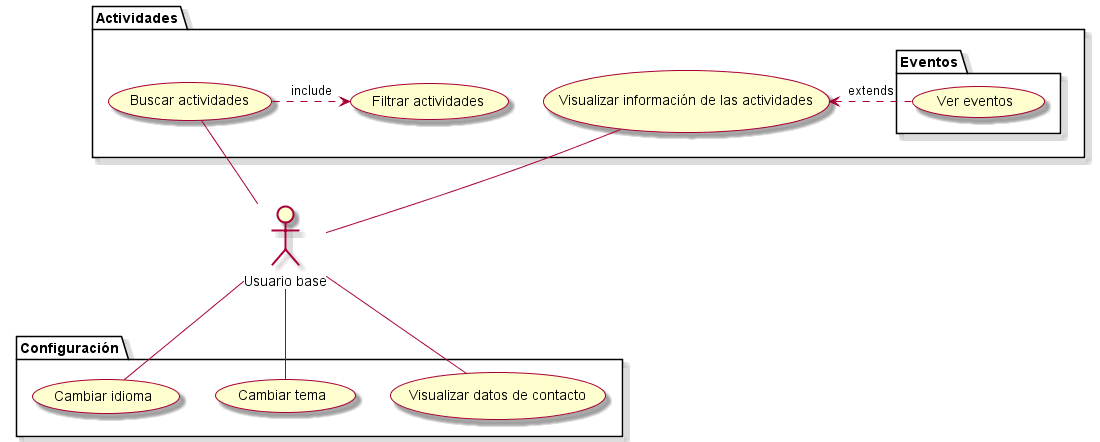
\includegraphics[width=1\linewidth]{5-AnalisisDelSistemaDeInformacion/Casos de uso/usuarioBase/diagrama.png}
	\caption{Diagrama - Usuario base}
\end{figure}
\begin{identificacionCasoDeUso}
	\begin{tabular} { | p{17cm} | }
		\hline
		Nombre del caso de uso                                                                                               \\ \hline
		Buscar actividades                                                                                                   \\ \hline
		Descripción del caso de uso                                                                                          \\ \hline
		Este caso de uso permite a cualquier usuario buscar actividades en el sistema aplicando ciertos filtros de búsqueda. \\ \hline
	\end{tabular}
	\caption{Caso de uso - Buscar actividades}
\end{identificacionCasoDeUso}
\begin{identificacionCasoDeUso}
	\begin{tabular} { | p{17cm} |}

		\hline
		Nombre del caso de uso                                                                                                         \\ \hline
		Visualizar información de las actividades                                                                                      \\ \hline
		Descripción del caso de uso                                                                                                    \\ \hline
		Este caso de uso permite a cualquier usuario ver información detallada sobre una actividad en particular, así como sus eventos \\ \hline
	\end{tabular}
	\caption{Caso de uso - Visualizar información de las actividades}
\end{identificacionCasoDeUso}
\begin{identificacionCasoDeUso}
	\begin{tabular} { | p{17cm} |}

		\hline
		Nombre del caso de uso                                                                                           \\ \hline
		Cambiar idioma                                                                                                   \\ \hline
		Descripción del caso de uso                                                                                      \\ \hline
		Este caso de uso permite a cualquier usuario cambiar el idioma de la aplicación entre inglés, español y francés. \\ \hline
	\end{tabular}
	\caption{Caso de uso - Cambiar idioma}
\end{identificacionCasoDeUso}
\begin{identificacionCasoDeUso}
	\begin{tabular} { | p{17cm} |}
		\hline
		Nombre del caso de uso                                                                                              \\ \hline
		Cambiar tema                                                                                                        \\ \hline
		Descripción del caso de uso                                                                                         \\ \hline
		Este caso de uso permite a cualquier usuario cambiar el tema de la aplicación entre el tema oscuro y el tema claro. \\ \hline
	\end{tabular}
	\caption{Caso de uso - Cambiar tema}
\end{identificacionCasoDeUso}
\begin{identificacionCasoDeUso}
	\begin{tabular} { | p{17cm} |}
		\hline
		Nombre del caso de uso                                                         \\ \hline
		Visualizar datos de contacto                                                   \\ \hline
		Descripción del caso de uso                                                    \\ \hline
		Este caso de uso permite a cualquier usuario visualizar los datos de contacto. \\ \hline
	\end{tabular}
	\caption{Caso de uso - Visualizar datos de contacto}
\end{identificacionCasoDeUso}
\subsubsection{Usuario no identificado}
\begin{figure}[H]
	\centering
	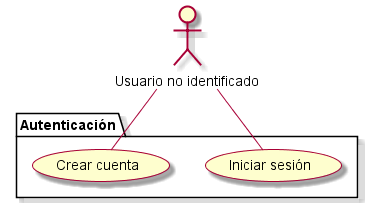
\includegraphics{5-AnalisisDelSistemaDeInformacion//Casos de uso//usuarioNoIdentificado//diagrama.png}
	\caption{Diagrama - Usuario no identificado}
\end{figure}
\begin{identificacionCasoDeUso}
	\begin{tabular} { | p{17cm} |}

		\hline
		Nombre del caso de uso               \\ \hline
		Crear cuenta                         \\ \hline
		Descripción del caso de uso          \\ \hline
		Este caso de uso permite a los usuarios no registrados, crearse una cuenta el sistema proporcionando la siguiente información:
		\begin{itemize}
			\item Nombre y apellidos del usuario
			\item Dirección de correo electronico
			\item Contraseña
			\item País (Opcional)
			\item Fecha de nacimiento (Opcional)
		\end{itemize} \\ \hline
	\end{tabular}
	\caption{Caso de uso - Crear cuenta}
\end{identificacionCasoDeUso}
\begin{identificacionCasoDeUso}
	\begin{tabular} { | p{17cm} |}

		\hline
		Nombre del caso de uso                                                                                                                  \\ \hline
		Iniciar sesión                                                                                                                          \\ \hline
		Descripción del caso de uso                                                                                                             \\ \hline
		Este caso de uso permite a los usuarios no registrados, iniciar sesión en el sistema proporcionando su correo electrónico y contraseña. \\ \hline
	\end{tabular}
	\caption{Caso de uso - Iniciar sesión}
\end{identificacionCasoDeUso}
\subsubsection{Usuario registrado}
\begin{figure}[H]
	\centering
	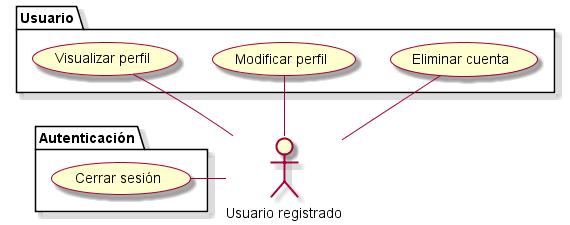
\includegraphics[width=1\linewidth]{5-AnalisisDelSistemaDeInformacion//Casos de uso//usuarioRegistrado/diagrama.png}
	\caption{Diagrama - Usuario registrado}
\end{figure}
\input{5-AnalisisDelSistemaDeInformacion/Casos de uso/usuarioRegistrado/Tablas/tablaCerrarSesión}
\begin{identificacionCasoDeUso}
	\begin{tabular} { | p{17cm} | }
		\hline
		Nombre del caso de uso                                                        \\ \hline
		Visualizar perfil                                                             \\ \hline
		Descripción del caso de uso                                                   \\ \hline
		Este caso de uso permite a los usuarios registrados, ver sus datos personales \\ \hline
	\end{tabular}
	\caption{Caso de uso - Visualizar perfil}
\end{identificacionCasoDeUso}
\begin{identificacionCasoDeUso}
	\begin{tabular} { | p{17cm} |}

		\hline
		Nombre del caso de uso                                                                                     \\ \hline
		Modificar perfil                                                                                           \\ \hline
		Descripción del caso de uso                                                                                \\ \hline
		Este caso de uso permite a los usuarios registrados, modificar su perfil actualizando sus datos personales \\ \hline
	\end{tabular}
	\caption{Caso de uso - Modificar perfil}
\end{identificacionCasoDeUso}
\begin{identificacionCasoDeUso}
	\begin{tabular} { | p{17cm} |}

		\hline
		Nombre del caso de uso                                                  \\ \hline
		Eliminar cuenta                                                         \\ \hline
		Descripción del caso de uso                                             \\ \hline
		Este caso de uso permite a los usuarios registrados, eliminar su cuenta \\ \hline
	\end{tabular}
	\caption{Caso de uso - Eliminar cuenta}
\end{identificacionCasoDeUso}
\subsubsection{Usuario registrado con rol de administrador}
\begin{figure}[H]
	\centering
	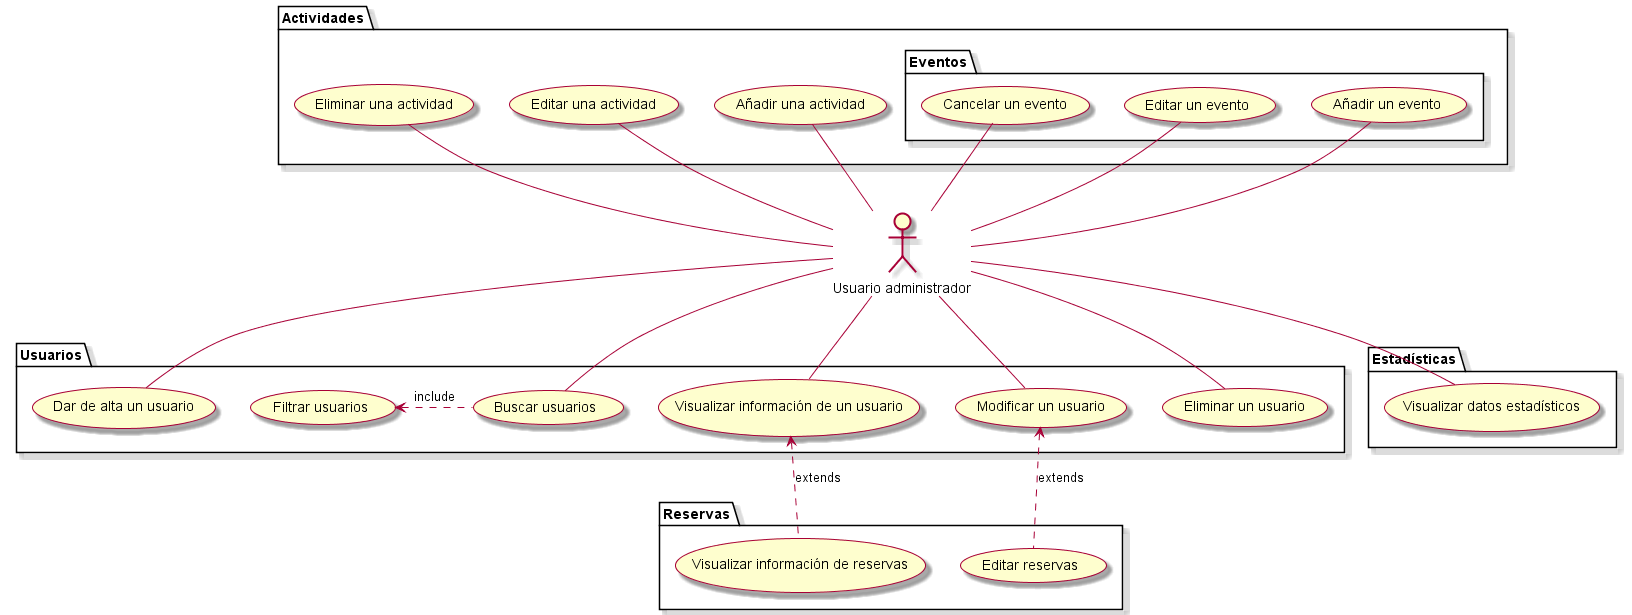
\includegraphics[width=1\linewidth]{5-AnalisisDelSistemaDeInformacion//Casos de uso//usuarioAdministrador/diagrama.png}
	\caption{Diagrama - Usuario administrador}
\end{figure}
\input{5-AnalisisDelSistemaDeInformacion/Casos de uso/usuarioAdministrador/Tablas/tablaAñadirActividad}
\begin{identificacionCasoDeUso}
	\begin{tabular} { | p{17cm} |}

		\hline
		Nombre del caso de uso                                                                                                                              \\ \hline
		Editar una actividad                                                                                                                                \\ \hline
		Descripción del caso de uso                                                                                                                         \\ \hline
		Este caso de uso permite a los usuarios registrados con el rol de administrador, editar la información de una actividad ya existente en el sistema. \\ \hline
	\end{tabular}
	\caption{Caso de uso - Editar una actividad}
\end{identificacionCasoDeUso}
\begin{identificacionCasoDeUso}
	\begin{tabular} { | p{17cm} |}

		\hline
		Nombre del caso de uso                                                                                                            \\ \hline
		Eliminar una actividad                                                                                                            \\ \hline
		Descripción del caso de uso                                                                                                       \\ \hline
		Este caso de uso permite a los usuarios registrados con el rol de administrador, eliminar una actividad ya existente del sistema. \\ \hline
	\end{tabular}
	\caption{Caso de uso - Eliminar una actividad}
\end{identificacionCasoDeUso}
\begin{identificacionCasoDeUso}
	\begin{tabular} { | p{17cm} |}

		\hline
		Nombre del caso de uso                  \\ \hline
		Dar de alta un usuario                  \\ \hline
		Descripción del caso de uso             \\ \hline
		Este caso de uso permite a los usuarios registrados con el rol de administrador, crear una nueva cuenta en el sistema proporcionando la siguiente información:
		\begin{itemize}
			\item Nombre y apellidos del usuario
			\item Dirección de correo electronico
			\item Role que tendrá dentro del sistema
			\item Contraseña
			\item Fecha de nacimiento (Opcional)
			\item Pais (Opcional)
		\end{itemize} \\ \hline
	\end{tabular}
	\caption{Caso de uso - Dar de alta un usuario}
\end{identificacionCasoDeUso}
\begin{identificacionCasoDeUso}
	\begin{tabular} { | p{17cm} |}

		\hline
		Nombre del caso de uso                                                                                                                                                  \\ \hline
		Buscar usuarios                                                                                                                                                         \\ \hline
		Descripción del caso de uso                                                                                                                                             \\ \hline
		Este caso de uso permite a los usuarios registrados con el rol de administrador, realizar búsquedas de usuarios en el sistema utilizando ciertos criterios de búsqueda. \\ \hline
	\end{tabular}
	\caption{Caso de uso - Buscar usuarios}
\end{identificacionCasoDeUso}
\input{5-AnalisisDelSistemaDeInformacion/Casos de uso/usuarioAdministrador/Tablas/tablaVisualizarInformaciónDeUsuario}
\begin{identificacionCasoDeUso}
	\begin{tabular} { | p{17cm} |}

		\hline
		Nombre del caso de uso                                                                                                                           \\ \hline
		Modificar un usuario                                                                                                                             \\ \hline
		Descripción del caso de uso                                                                                                                      \\ \hline
		Este caso de uso permite a los usuarios registrados con el rol de administrador, editar la información de un usuario ya existente en el sistema. \\ \hline
	\end{tabular}
	\caption{Caso de uso - Modificar un usuario}
\end{identificacionCasoDeUso}
\begin{identificacionCasoDeUso}
	\begin{tabular} { | p{17cm} |}

		\hline
		Nombre del caso de uso                                                                                                         \\ \hline
		Eliminar un usuario                                                                                                            \\ \hline
		Descripción del caso de uso                                                                                                    \\ \hline
		Este caso de uso permite a los usuarios registrados con el rol de administrador, eliminar un usuario ya existente del sistema. \\ \hline
	\end{tabular}
	\caption{Caso de uso - Eliminar un usuario}
\end{identificacionCasoDeUso}
\begin{identificacionCasoDeUso}
	\begin{tabular} { | p{17cm} |}
		\hline
		Nombre del caso de uso                       \\ \hline
		Añadir un evento                             \\ \hline
		Descripción del caso de uso                  \\ \hline
		Este caso de uso permite a los usuarios registrados con el rol de administrador, crear un evento de una actividad ya existente en el sistema. Se deberá proporcionar la siguiente información:
		\begin{itemize}
			\item Número de plazas totales a publicar
			\item Idioma en el que se impartirá el evento
			\item Guía asignado
			\item Día y hora del comienzo del evento
		\end{itemize} \\ \hline
	\end{tabular}
	\caption{Caso de uso - Añadir un evento}
\end{identificacionCasoDeUso}
\begin{identificacionCasoDeUso}
	\begin{tabular} { | p{17cm} |}

		\hline
		Nombre del caso de uso                                                                                                                          \\ \hline
		Editar un evento                                                                                                                                \\ \hline
		Descripción del caso de uso                                                                                                                     \\ \hline
		Este caso de uso permite a los usuarios registrados con el rol de administrador, editar la información de un evento ya existente en el sistema. \\ \hline
	\end{tabular}
	\caption{Caso de uso - Editar un evento}
\end{identificacionCasoDeUso}
\begin{identificacionCasoDeUso}
	\begin{tabular} { | p{17cm} |}

		\hline
		Nombre del caso de uso                                                                                                                                  \\ \hline
		Cancelar un evento                                                                                                                                      \\ \hline
		Descripción del caso de uso                                                                                                                             \\ \hline
		Este caso de uso permite a los usuarios registrados con el rol de administrador, cancelar un evento ya existente y que no esté cancelado en el sistema. \\ \hline
	\end{tabular}
	\caption{Caso de uso - Cancelar un evento}
\end{identificacionCasoDeUso}
\begin{identificacionCasoDeUso}
	\begin{tabular} { | p{17cm} |}

		\hline
		Nombre del caso de uso                                                                                                                     \\ \hline
		Visualizar datos estadísticos                                                                                                              \\ \hline
		Descripción del caso de uso                                                                                                                \\ \hline
		Este caso de uso permite a los usuarios registrados con el rol de administrador, visualizar datos estadísticos de las reservas y usuarios. \\ \hline
	\end{tabular}
	\caption{Caso de uso - Visualizar datos estadísticos}
\end{identificacionCasoDeUso}
\subsubsection{Usuario registrado con rol de guía}
\begin{figure}[H]
	\centering
	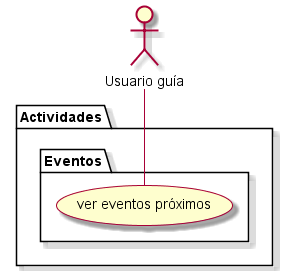
\includegraphics{5-AnalisisDelSistemaDeInformacion//Casos de uso//usuarioGuia/diagrama.png}
	\caption{Diagrama - Usuario guía}
\end{figure}
\begin{identificacionCasoDeUso}
	\begin{tabular} { | p{17cm} |}

		\hline
		Nombre del caso de uso                                                                                                            \\ \hline
		Ver eventos próximos                                                                                                              \\ \hline
		Descripción del caso de uso                                                                                                       \\ \hline
		Este caso de uso permite a los usuarios registrados con rol de guía, obtener un listado de todos los eventos que tiene asignados. \\ \hline
	\end{tabular}
	\caption{Caso de uso - Ver eventos próximos}
\end{identificacionCasoDeUso}
\subsubsection{Usuario registrado con rol de turista}
\begin{figure}[H]
	\centering
	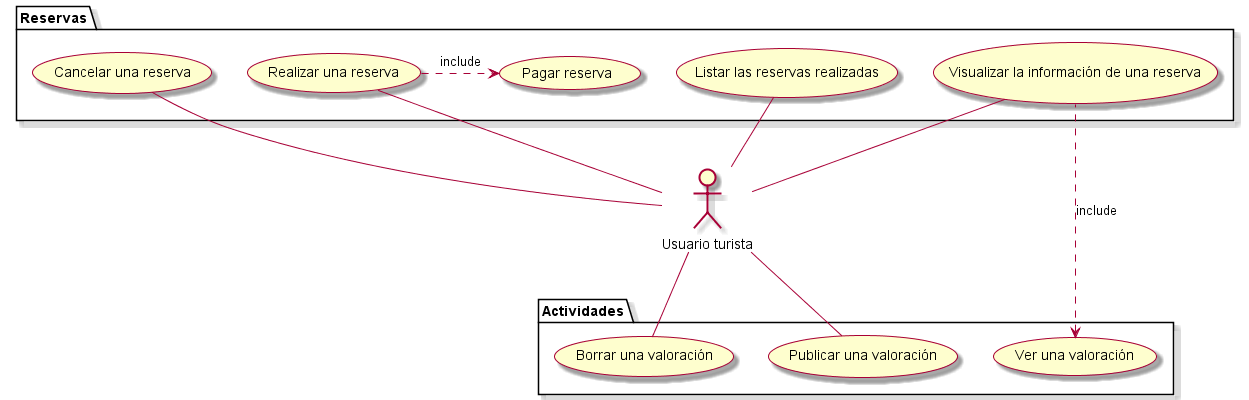
\includegraphics[width=1\linewidth]{5-AnalisisDelSistemaDeInformacion//Casos de uso//usuarioTurista/diagrama.png}
	\caption{Diagrama - Usuario turista}
\end{figure}
\begin{identificacionCasoDeUso}
	\begin{tabular} { | p{17cm} |}

		\hline
		Nombre del caso de uso                                                                                            \\ \hline
		Realizar una reserva                                                                                              \\ \hline
		Descripción del caso de uso                                                                                       \\ \hline
		Este caso de uso permite a los usuarios registrados con el rol de turista, realizar una reserva de una actividad. \\ \hline
	\end{tabular}
	\caption{Caso de uso - Realizar una reserva}
\end{identificacionCasoDeUso}
\begin{identificacionCasoDeUso}
	\begin{tabular} { | p{17cm} |}

		\hline
		Nombre del caso de uso                                                                                                                                \\ \hline
		Cancelar una reserva                                                                                                                                  \\ \hline
		Descripción del caso de uso                                                                                                                           \\ \hline
		Este caso de uso permite a los usuarios registrados con el rol turista, cancelar una reserva ya confirmada, 24 horas antes del inicio de la actividad \\ \hline
	\end{tabular}
	\caption{Caso de uso - Cancelar una reserva}
\end{identificacionCasoDeUso}
\input{5-AnalisisDelSistemaDeInformacion/Casos de uso/usuarioTurista/Tablas/tablaPublicarValoración}
\begin{identificacionCasoDeUso}
	\begin{tabular} { | p{17cm} |}

		\hline
		Nombre del caso de uso                                                                                            \\ \hline
		Borrar una valoración                                                                                             \\ \hline
		Descripción del caso de uso                                                                                       \\ \hline
		Este caso de uso permite a los usuarios registrados con el rol turista, eliminar la valoración que haya publicado \\ \hline
	\end{tabular}
	\caption{Caso de uso - Borrar una valoración}
\end{identificacionCasoDeUso}
\begin{identificacionCasoDeUso}
	\begin{tabular} { | p{17cm} |}

		\hline
		Nombre del caso de uso                                                                                                               \\ \hline
		Listar las reservas realizadas                                                                                                       \\ \hline
		Descripción del caso de uso                                                                                                          \\ \hline
		Este caso de uso permite a los usuarios registrados con el rol de turista, listar todas las reservas realizadas a modo de historial. \\ \hline
	\end{tabular}
	\caption{Caso de uso - Listar las reservas realizadas}
\end{identificacionCasoDeUso}
\input{5-AnalisisDelSistemaDeInformacion/Casos de uso/usuarioTurista/Tablas/tablaVerInformaciónDeLaReserva}

\section{Identificación de Subsistemas}
\subsection{Descripción de los subsistemas}
\subsubsection{Subsistema de gestión de usuarios}
Este subsistema se encarga de todas las operaciones relacionadas con los usuarios de la aplicación. Permite al administrador realizar funciones como la creación, edición, eliminación y listado de usuarios. Además, cualquier usuario puede registrarse, iniciar y cerrar sesión, así como editar su propio perfil.
\subsubsection{Subsistema de gestión de actividades}
Responsable de las operaciones vinculadas a las actividades, este subsistema permite al administrador crear, editar, listar y eliminar actividades. Los usuarios pueden acceder a la información relacionada con cada actividad, incluyendo valoraciones y eventos.
\subsubsection{Subsistema de gestión de reservas}
Este subsistema maneja todas las operaciones relacionadas con las reservas. Los usuarios registrados pueden crear, modificar, cancelar y listar sus reservas. El administrador tiene la capacidad de listar y editar las reservas realizadas por los usuarios.
\subsection*{Descripción de los interfaces entre subsistemas}
\begin{figure}[H]
	\centering
	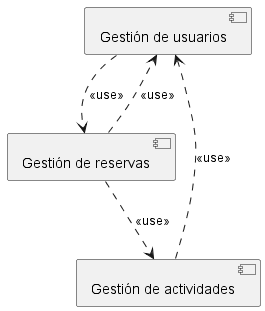
\includegraphics[width=0.5\linewidth]{5-AnalisisDelSistemaDeInformacion/diagrama.png}
	\caption{Diagrama de las relaciones entre los subsistemas}
	\label{fig:diagrama}
\end{figure}
El subsistema de gestión de usuarios interactúa con el subsistema de reservas para obtener las reservas asociadas a un usuario. A su vez, el subsistema de reservas se comunica con el subsistema de usuarios para crear una reserva vinculada a un usuario específico. Este proceso también implica al subsistema de actividades, que recibe información del subsistema de reservas para asociar la actividad que el usuario desea reservar. Finalmente, el subsistema de actividades llama al subsistema de usuarios para asignar un guía a las actividades programadas.
\section{Análisis de los casos de uso}
\subsection{Buscar actividades}
El caso de uso “Buscar actividades” describe cómo los usuarios interactúan con la aplicación para buscar actividades basadas en diferentes criterios.
\begin{analisisCasoDeUso}
	\centering
	\begin{tabular} { | m{3cm} | p{13cm} | }
		\hline
		\multicolumn{2}{ | c | }{\bfseries Buscar actividades}                                                                                                                         \\ \hline
		{\bfseries Precondiciones}  & No.                                                                                                                                              \\ \hline
		{\bfseries Postcondiciones} & Se muestra una lista de actividades que coinciden con los criterios de búsqueda.                                                                 \\ \hline
		{\bfseries Actores    }     & Iniciado por cualquier usuario ya esté identificado o no.                                                                                        \\ \hline
		{\bfseries Descripción}     & {\bfseries 1.} El usuario accede al apartado de búsqueda de actividades en la aplicación.                                                        \\
		                            & {\bfseries 2.} El usuario introduce texto en la barra de búsqueda para filtrar actividades por nombre y ubicación.                               \\
		                            & {\bfseries 3.} El sistema espera a que se deje de escribir para hacer la búsqueda.                                                               \\
		                            & {\bfseries 4.} El sistema muestra una lista de actividades que coinciden con los criterios de búsqueda aplicados.                                \\
		                            & {\bfseries 5.} El usuario puede desplazarse por la lista para ver las actividades que cumplen con los criterios de búsqueda especificados.       \\ \hline
		{\bfseries Variaciones}     & {\bfseries Escenario Alternativo 1:} El usuario realiza una búsqueda sin especificar ningún criterio.                                            \\
		                            & {\bfseries 1.} El usuario accede al apartado de búsqueda de actividades en la aplicación.                                                        \\
		                            & {\bfseries 2.} El sistema muestra la lista de actividades más populares.                                                                         \\
		                            & {\bfseries 3.} Volver al paso 5.                                                                                                                 \\
		                            & {\bfseries Escenario Alternativo 2:} El usuario realiza una búsqueda utilizando los filtros para refinar la búsqueda según fechas, precios, etc. \\
		                            & {\bfseries 1.} El usuario accede al apartado de búsqueda de actividades en la aplicación.                                                        \\
		                            & {\bfseries 2.} El usuario añade filtros de fechas, precios, etc.                                                                                 \\
		                            & {\bfseries 3.} Volver al paso 4.                                                                                                                 \\
		                            & {\bfseries Escenario Alternativo 3:} El sistema no encuentra ninguna actividad que coincida con los criterios de búsqueda.                       \\
		                            & {\bfseries 4.} El sistema muestra un mensaje pidiendo al usuario que cambie los criterios de búsqueda                                            \\ \hline
		{\bfseries Excepciones}     & Si ocurre un error al acceder a la base de datos, se muestra un mensaje de error.                                                                \\ \hline
		{\bfseries Notas }          &                                                                                                                                                  \\ \hline
	\end{tabular}
	\caption{Caso de uso - Buscar actividades}
\end{analisisCasoDeUso}

\subsection{Visualizar información de las actividades}
El caso de uso “Visualizar información de las actividades” describe cómo los usuarios pueden acceder a detalles específicos sobre una actividad seleccionada.
\begin{analisisCasoDeUso}
	\centering
	\begin{tabular} { | m{3cm} | p{13cm} | }
		\hline
		\multicolumn{2}{ | c | }{\bfseries Visualizar información de actividades}                                                                                                         \\ \hline
		{\bfseries Precondiciones}  & No.                                                                                                                                                 \\ \hline
		{\bfseries Postcondiciones} & Se muestra la información detallada de una actividad específica.                                                                                    \\ \hline
		{\bfseries Actores    }     & Iniciado por cualquier usuario ya esté identificado o no.                                                                                           \\ \hline
		{\bfseries Descripción}     & {\bfseries 1.} El usuario selecciona una actividad de la lista de resultados o desde otra parte de la aplicación.                                   \\
		                            & {\bfseries 2.} El sistema muestra la información detallada de la actividad seleccionada, incluyendo descripción, imágenes, ubicación, precios, etc. \\
		                            & {\bfseries 3.} El usuario puede explorar la información.                                                                                            \\ \hline
		{\bfseries Variaciones}     & {\bfseries Escenario alternativo 1:} Actividad eliminada o no disponible.                                                                           \\
		                            & {\bfseries 2.} El sistema muestra un mensaje de error.                                                                                              \\ \hline
		{\bfseries Excepciones}     & Si ocurre un error al acceder a la base de datos, se muestra un mensaje de error.                                                                   \\ \hline
		{\bfseries Notas }          &                                                                                                                                                     \\ \hline
	\end{tabular}
	\caption{Caso de uso - Visualizar información de actividades}
\end{analisisCasoDeUso}
\subsection{Cambiar idioma}
El caso de uso “Cambiar idioma” permite a los usuarios seleccionar el idioma en el que prefieren visualizar la aplicación.
\begin{analisisCasoDeUso}
	\centering
	\begin{tabular} { | m{3cm} | p{13cm} | }
		\hline
		\multicolumn{2}{ | c | }{\bfseries Cambiar idioma}                                                                               \\ \hline
		{\bfseries Precondiciones}  & En caso de estar en la aplicación web, tener las cookies habilitadas en el navegador.              \\ \hline
		{\bfseries Postcondiciones} & Se muestra la aplicación en el idioma seleccionado.                                                \\ \hline
		{\bfseries Actores    }     & Iniciado por cualquier usuario ya esté identificado o no.                                          \\ \hline
		{\bfseries Descripción}     & {\bfseries 1.} El usuario selecciona en el menú la opción para cambiar el idioma de la aplicación. \\
		                            & {\bfseries 2.} El sistema muestra una lista de idiomas disponibles.                                \\
		                            & {\bfseries 3.} El usuario selecciona el idioma deseado.                                            \\
		                            & {\bfseries 4.} El sistema actualiza el idioma de la aplicación según la selección del usuario.     \\
		                            & {\bfseries 5.} El usuario puede ver la aplicación con el idioma cambiado.                          \\ \hline
		{\bfseries Variaciones}     & No.                                                                                                \\ \hline
		{\bfseries Excepciones}     & Si ocurre un error en el proceso de cambio de idioma, se muestra un mensaje de error.              \\ \hline
		{\bfseries Notas }          &                                                                                                    \\ \hline
	\end{tabular}
	\caption{Caso de uso - Cambiar idioma}
\end{analisisCasoDeUso}

\subsection{Cambiar tema}
El caso de uso “Cambiar tema” permite a los usuarios cambiar la apariencia de la aplicación seleccionando diferentes temas.
\begin{analisisCasoDeUso}
	\centering
	\begin{tabular} { | m{3cm} | p{13cm} | }
		\hline
		\multicolumn{2}{ | c | }{\bfseries Cambiar tema}                                                                                         \\ \hline
		{\bfseries Precondiciones}  & En caso de estar en la aplicación web, tener las cookies habilitadas en el navegador.                      \\ \hline
		{\bfseries Postcondiciones} & Se muestra la aplicación en el tema seleccionado.                                                          \\ \hline
		{\bfseries Actores    }     & Iniciado por cualquier usuario ya esté identificado o no.                                                  \\ \hline
		{\bfseries Descripción}     & {\bfseries 1.} El usuario selecciona en el menú la opción para cambiar el tema de la aplicación.           \\
		                            & {\bfseries 2.} El sistema cambia el tema de la aplicación según el tema que estaba aplicado anteriormente. \\
		                            & {\bfseries 3.} El usuario puede ver la aplicación con el tema cambiado.                                    \\ \hline
		{\bfseries Variaciones}     & No.                                                                                                        \\ \hline
		{\bfseries Excepciones}     & Si ocurre un error en el proceso de cambio de tema, se muestra un mensaje de error.                        \\ \hline
		{\bfseries Notas }          &                                                                                                            \\ \hline
	\end{tabular}
	\caption{Caso de uso - Cambiar tema}
\end{analisisCasoDeUso}

\subsection{Visualizar datos de contacto}
El caso de uso “Visualizar datos de contacto” permite a los usuarios acceder a la información de contacto almacenada en el sistema.
\begin{analisisCasoDeUso}
	\centering
	\begin{tabular} { | m{3cm} | p{13cm} | }
		\hline
		\multicolumn{2}{ | c | }{\bfseries Visualizar datos de contacto}                                                \\ \hline
		{\bfseries Precondiciones}  & No.                                                                               \\ \hline
		{\bfseries Postcondiciones} & El usuario desea visualizar los datos de contacto.                                \\ \hline
		{\bfseries Actores    }     & Iniciado por cualquier usuario ya esté identificado o no.                         \\ \hline
		{\bfseries Descripción}     & 1. El usuario accede a cualquier página del sistema.                              \\
		                            & 2. El sistema muestra los datos de contacto en el pie de la página.               \\ \hline
		{\bfseries Variaciones}     & No.                                                                                \\ \hline
		{\bfseries Excepciones}     & Si ocurre un error al acceder a la base de datos, se muestra un mensaje de error. \\ \hline
		{\bfseries Notas }          &                                                                                   \\ \hline
	\end{tabular}
	\caption{Caso de uso - Visualizar datos de contacto}
\end{analisisCasoDeUso}


\subsection{Crear cuenta}
El caso de uso “Crear cuenta” describe el proceso mediante el cual un nuevo usuario puede registrarse en el sistema
\begin{analisisCasoDeUso}
	\centering
	\begin{tabular} { | m{3cm} | p{13cm} | }
		\hline
		\multicolumn{2}{ | c | }{\bfseries Crear cuenta}                                                                        \\ \hline
		{\bfseries Precondiciones}  & No.                                                                                       \\ \hline
		{\bfseries Postcondiciones} & El usuario queda registrado en el sistema e inicia sesión automáticamente.                \\ \hline
		{\bfseries Actores    }     & Iniciado por cualquier usuario sin identificar                                            \\ \hline
		{\bfseries Descripción}     & {\bfseries 1.} El usuario selecciona en el menú la opción “Cuenta” .                       \\
		                            & {\bfseries 2.} El sistema muestra la página de inicio de sesión.                          \\
		                            & {\bfseries 3.} El usuario selecciona la opción “Regístrate aquí” .                         \\
		                            & {\bfseries 4.} El sistema muestra la página de registro.                                  \\
		                            & {\bfseries 5.} El usuario introduce los datos requeridos.                                 \\
		                            & {\bfseries 6.} El usuario envía el formulario de registro.                                \\
		                            & {\bfseries 7.} El sistema valida los datos del formulario.                                \\
		                            & {\bfseries 8.} El sistema registra los datos del usuario en la base de datos.             \\
		                            & {\bfseries 9.} El sistema confirma el registro del usuario.                               \\ \hline
		{\bfseries Variaciones}     & {\bfseries Escenario alternativo 1:} En caso de que los datos ingresados no sean válidos. \\
		                            & {\bfseries 8.} El sistema muestra un mensaje de error.                                    \\
		                            & {\bfseries Volver al paso 4.}                                                             \\ \hline
		{\bfseries Excepciones}     & Si ocurre un error en el proceso de registro, se muestra un mensaje de error.             \\ \hline
		{\bfseries Notas }          &                                                                                           \\ \hline
	\end{tabular}
	\caption{Caso de uso - Crear cuenta}
\end{analisisCasoDeUso}
\subsection{Iniciar sesión}
El caso de uso “Iniciar sesión” permite a los usuarios registrados acceder a sus cuentas en el sistema.
\begin{analisisCasoDeUso}
	\centering
	\begin{tabular} { | m{3cm} | p{13cm} | }
		\hline
		\multicolumn{2}{ | c | }{\bfseries Iniciar sesión}                                                                       \\ \hline
		{\bfseries Precondiciones}  & El usuario debe haberse creado una cuenta en el sistema.                                   \\ \hline
		{\bfseries Postcondiciones} & El usuario queda identificado.                                                             \\ \hline
		{\bfseries Actores    }     & Iniciado por cualquier usuario sin identificar                                             \\ \hline
		{\bfseries Descripción}     & {\bfseries 1.} El usuario selecciona en el menú la opción “Área Personal” .                 \\
		                            & {\bfseries 2.} El sistema muestra la página de inicio de sesión.                           \\
		                            & {\bfseries 3.} El usuario introduce los datos requeridos.                                  \\
		                            & {\bfseries 4.} El usuario envía el formulario de registro.                                 \\
		                            & {\bfseries 5.} El sistema verifica los datos del formulario.                               \\
		                            & {\bfseries 6.} El usuario queda identificado.                                              \\ \hline
		{\bfseries Variaciones}     & {\bfseries Escenario alternativo 1:} En caso de que los datos ingresados sean incorrectos. \\
		                            & {\bfseries 6.} El sistema muestra un mensaje de error.                                     \\ \hline
		{\bfseries Excepciones}     & Si ocurre un error en el proceso de inicio de sesión, se muestra un mensaje de error.      \\
		{\bfseries Notas }          &                                                                                            \\ \hline
	\end{tabular}
	\caption{Caso de uso - Iniciar sesión}
\end{analisisCasoDeUso}
\subsection{Cerrar sesión}
El caso de uso “Cerrar sesión” describe el proceso mediante el cual un usuario puede salir de su cuenta en el sistema de manera segura.
\begin{analisisCasoDeUso}
	\centering
	\begin{tabular} { | m{3cm} | p{13cm} | }
		\hline
		\multicolumn{2}{ | c | }{\bfseries Cerrar sesión}                                                                   \\ \hline
		{\bfseries Precondiciones}  & No.                                                                                   \\ \hline
		{\bfseries Postcondiciones} & El usuario cierra sesión en el sistema.                                               \\ \hline
		{\bfseries Actores    }     & Iniciado por cualquier usuario identificado.                                          \\ \hline
		{\bfseries Descripción}     & {\bfseries 1.} El usuario selecciona en el menú la opción “Área Personal” .            \\
		                            & {\bfseries 2.} El sistema muestra la página de perfil.                                \\
		                            & {\bfseries 3.} El usuario visualiza la información de su perfil.                      \\
		                            & {\bfseries 4.} El usuario selecciona la opción “Cerrar sesión” .                       \\
		                            & {\bfseries 5.} El sistema cierra la sesión del usuario.                               \\ \hline
		{\bfseries Variaciones}     & No.                                                                                   \\ \hline
		{\bfseries Excepciones}     & Si ocurre un error en el proceso de cierre de sesión, se muestra un mensaje de error. \\ \hline
		{\bfseries Notas }          &                                                                                       \\ \hline
	\end{tabular}
	\caption{Caso de uso - Cerrar sesión}
\end{analisisCasoDeUso}
\subsection{Visualizar perfil}
El caso de uso “Visualizar perfil” permite a los usuarios acceder y ver la información de su perfil personal.
\begin{analisisCasoDeUso}
	\centering
	\begin{tabular} { | m{3cm} | p{13cm} | }
		\hline
		\multicolumn{2}{ | c | }{\bfseries Visualizar perfil}                                                    \\ \hline
		{\bfseries Precondiciones}  & No.                                                                        \\ \hline
		{\bfseries Postcondiciones} & Se muestra la información del perfil del usuario.                          \\ \hline
		{\bfseries Actores    }     & Iniciado por cualquier usuario identificado.                               \\ \hline
		{\bfseries Descripción}     & {\bfseries 1.} El usuario selecciona en el menú la opción “Área Personal” . \\
		                            & {\bfseries 2.} El sistema muestra la página de perfil.                     \\
		                            & {\bfseries 3.} El usuario visualiza la información de su perfil.           \\ \hline
		{\bfseries Variaciones}     & No.                                                                        \\ \hline
		{\bfseries Excepciones}     & Si ocurre un error en la base de datos, se muestra un mensaje de error.    \\ \hline
		{\bfseries Notas }          &                                                                            \\ \hline
	\end{tabular}
	\caption{Caso de uso - Visualizar perfil}
\end{analisisCasoDeUso}
\subsection{Modificar perfil}
El caso de uso “Modificar perfil” permite a los usuarios editar y actualizar la información de su perfil personal.
\begin{analisisCasoDeUso}
	\centering
	\begin{tabular} { | m{3cm} | p{13cm} | }
		\hline
		\multicolumn{2}{ | c | }{\bfseries Modificar perfil}                                                                   \\ \hline
		{\bfseries Precondiciones}  & No.                                                                                      \\ \hline
		{\bfseries Postcondiciones} & Los cambios realizados en el perfil del usuario son guardados.                           \\ \hline
		{\bfseries Actores    }     & Iniciado por cualquier usuario identificado.                                             \\ \hline
		{\bfseries Descripción}     & {\bfseries 1.} El usuario selecciona en el menú la opción “Área Personal” .               \\
		                            & {\bfseries 2.} El sistema muestra la página de perfil.                                   \\
		                            & {\bfseries 3.} El usuario visualiza la información de su perfil.                         \\
		                            & {\bfseries 4.} El usuario selecciona la opción “Editar datos de perfil” .                 \\
		                            & {\bfseries 5.} El sistema muestra un formulario con los datos del perfil del usuario.    \\
		                            & {\bfseries 6.} El usuario realiza los cambios deseados en la información del perfil.     \\
		                            & {\bfseries 7.} El usuario guarda los cambios.                                            \\
		                            & {\bfseries 8.} El sistema valida los nuevos datos del perfil.                            \\
		                            & {\bfseries 9.} El sistema actualiza los datos del usuario en el sistema.                 \\ \hline
		{\bfseries Variaciones}     & {\bfseries Escenario alternativo 1:} En caso de que los datos cambiados no sean válidos. \\
		                            & {\bfseries 9.} El sistema muestra un mensaje de error.                                   \\
		                            & {\bfseries 10.} Volver al paso 3.                                                        \\
		                            & {\bfseries Escenario alternativo 2:} En caso de que no se quiera hacer un cambio.        \\
		                            & {\bfseries 7.} El usuario cancela la edición.                                            \\
		                            & {\bfseries 8.} El usuario visualiza la información de su perfil.                         \\ \hline
		{\bfseries Excepciones}     & Si ocurre un error en el proceso de edición del perfil, se muestra un mensaje de error.  \\ \hline
		{\bfseries Notas }          &                                                                                          \\ \hline
	\end{tabular}
	\caption{Caso de uso - Modificar perfil}
\end{analisisCasoDeUso}
\subsection{Eliminar cuenta}
El caso de uso “Eliminar cuenta” describe el proceso mediante el cual un usuario puede eliminar su cuenta del sistema.
\begin{analisisCasoDeUso}
	\centering
	\begin{tabular} { | m{3cm} | p{13cm} | }
		\hline
		\multicolumn{2}{ | c | }{\bfseries Eliminar cuenta}                                                                      \\ \hline
		{\bfseries Precondiciones}  & El usuario debe estar identificado.                                                        \\ \hline
		{\bfseries Postcondiciones} & La cuenta del usuario es eliminada del sistema y se cierra sesión en el sistema.           \\ \hline
		{\bfseries Actores    }     & Usuario                                                                                    \\ \hline
		{\bfseries Descripción}     & {\bfseries 1.} El usuario selecciona en el menú la opción “Área Personal” .                 \\
		                            & {\bfseries 2.} El sistema muestra la página de perfil.                                     \\
		                            & {\bfseries 3.} El usuario visualiza la información de su perfil.                           \\
		                            & {\bfseries 4.} El usuario selecciona la opción “Eliminar Cuenta” .                          \\
		                            & {\bfseries 5.} El sistema pide confirmación.                                               \\
		                            & {\bfseries 6.} El usuario confirma la eliminación                                          \\
		                            & {\bfseries 7.} El sistema elimina la cuenta.                                               \\
		                            & {\bfseries 8.} El sistema cierra la sesión del usuario.                                    \\ \hline
		{\bfseries Variaciones}     & {\bfseries Escenario alternativo 1:} En caso de que se cancele la eliminación              \\
		                            & {\bfseries 6.} El usuario cancela la eliminación                                           \\
		                            & {\bfseries 7.} El sistema cancela la eliminación                                           \\ \hline
		{\bfseries Excepciones}     & Si ocurre un error en el proceso de eliminación de cuenta, se muestra un mensaje de error. \\ \hline
		{\bfseries Notas }          &                                                                                            \\ \hline
	\end{tabular}
	\caption{Caso de uso - Eliminar cuenta}
\end{analisisCasoDeUso}
\subsection{Añadir una actividad}
El caso de uso “Añadir una actividad” permite a los administradores del sistema agregar nuevas actividades al sistema.
\begin{analisisCasoDeUso}
	\centering
	\begin{tabular} { | m{3cm} | p{13cm} | }
		\hline
		\multicolumn{2}{ | c | }{\bfseries Añadir una actividad}                                                                           \\ \hline
		{\bfseries Precondiciones}  & Estar accediendo a la aplicación a través de un ordenador.                                           \\ \hline
		{\bfseries Postcondiciones} & Registrar en el sistema una nueva actividad.                                                         \\ \hline
		{\bfseries Actores    }     & Iniciado por cualquier usuario con rol administrador.                                                \\ \hline
		{\bfseries Descripción}     & {\bfseries 1.} El usuario selecciona en el menú la opción “Dashboard” .                               \\
		                            & {\bfseries 2.} El sistema muestra la pantalla principal del dashboard junto a un menú lateral.       \\
		                            & {\bfseries 3.} El usuario selecciona en el menú lateral la opción “Actividades” .                     \\
		                            & {\bfseries 4.} El sistema muestra un listado de actividades ya existentes.                           \\
		                            & {\bfseries 5.} El usuario selecciona el botón “Añadir actividad” .                                    \\
		                            & {\bfseries 6.} El sistema muestra un formulario.                                                     \\
		                            & {\bfseries 7.} El usuario introduce los datos requeridos.                                            \\
		                            & {\bfseries 8.} El usuario envía el formulario de creación de actividad.                              \\
		                            & {\bfseries 9.} El sistema verifica los datos del formulario.                                         \\
		                            & {\bfseries 10.} El sistema registra los datos de la nueva actividad en la base de datos.             \\\hline
		{\bfseries Variaciones}     & {\bfseries Escenario Alternativo 1} El usuario cancela la creación de la nueva actividad             \\
		                            & {\bfseries 8.} El usuario presiona la opción “Cerrar”.                                               \\
		                            & {\bfseries 9.} El sistema cierra el formulario.                                                      \\
		                            & {\bfseries Escenario Alternativo 2} El usuario no rellena correctamente el formulario.               \\
		                            & {\bfseries 10.} El sistema muestra un mensaje de error                                               \\
		                            & {\bfseries 11.} Volver al paso 7.                                                                    \\ \hline
		{\bfseries Excepciones}     & Si ocurre un error en el proceso de creación de una nueva actividad, se muestra un mensaje de error. \\ \hline
		{\bfseries Notas }          &                                                                                                      \\ \hline
	\end{tabular}
	\caption{Caso de uso - Añadir una actividad}
\end{analisisCasoDeUso}
\subsection{Editar una actividad}
El caso de uso “Editar una actividad” describe cómo los administradores pueden modificar la información de las actividades existentes en el sistema.
\begin{analisisCasoDeUso}
	\centering
	\begin{tabular} { | m{3cm} | p{13cm} | }
		\hline
		\multicolumn{2}{ | c | }{\bfseries Editar una actividad}                                                                     \\ \hline
		{\bfseries Precondiciones}  & Debe haber actividades registradas.                                                            \\ \hline
		{\bfseries Postcondiciones} & La actividad refleja los cambios realizados                                                    \\ \hline
		{\bfseries Actores    }     & Usuario identificado con rol administrador.                                                    \\ \hline
		{\bfseries Descripción}     & {\bfseries 1.} El usuario selecciona en el menú la opción “Dashboard” .                         \\
		                            & {\bfseries 2.} El sistema muestra la pantalla principal del dashboard junto a un menú lateral. \\
		                            & {\bfseries 3.} El usuario selecciona en el menú lateral la opción “Actividades” .               \\
		                            & {\bfseries 4.} El sistema muestra un listado de actividades ya existentes.                     \\
		                            & {\bfseries 5.} El usuario selecciona la opción “Editar” de la actividad que quiere editar.     \\
		                            & {\bfseries 6.} El usuario realiza los cambios deseados.                                        \\
		                            & {\bfseries 7.} El sistema valida los datos.                                                    \\
		                            & {\bfseries 8.} El sistema actualiza la actividad.                                              \\ \hline
		{\bfseries Variaciones}     & {\bfseries Escenario alternativo 1:} Si los datos ingresados son incorrectos.                  \\
		                            & {\bfseries 8.} El sistema muestra un mensaje de error.                                         \\
		                            & {\bfseries 9.} Vuelve al paso 6.                                                               \\ \hline
		{\bfseries Excepciones}     & Si ocurre un error en el proceso de edición, se muestra un mensaje de error.                   \\ \hline
		{\bfseries Notas }          &                                                                                                \\ \hline
	\end{tabular}
	\caption{Caos de uso - Editar una actividad}
\end{analisisCasoDeUso}
\subsection{Eliminar una actividad}
El caso de uso “Eliminar una actividad” permite a los administradores eliminar actividades del sistema.
\begin{analisisCasoDeUso}
	\centering
	\begin{tabular} { | m{3cm} | p{13cm} | }
		\hline
		\multicolumn{2}{ | c | }{\bfseries Eliminar una actividad}                                                                   \\ \hline
		{\bfseries Precondiciones}  & Debe haber actividades registradas.                                                            \\ \hline
		{\bfseries Postcondiciones} & Se eliminan actividades previamente registradas.                                               \\ \hline
		{\bfseries Actores    }     & Usuario identificado con rol administrador.                                      \\ \hline
		{\bfseries Descripción}     & {\bfseries 1.} El usuario selecciona en el menú la opción “Dashboard” .                         \\
		                            & {\bfseries 2.} El sistema muestra la pantalla principal del dashboard junto a un menú lateral. \\
		                            & {\bfseries 3.} El usuario selecciona en el menú lateral la opción “Actividades” .               \\
		                            & {\bfseries 4.} El sistema muestra un listado de actividades ya existentes.                     \\
		                            & {\bfseries 5.} El usuario selecciona la opción “Eliminar” de la actividad que quiere eliminar. \\
		                            & {\bfseries 6.} El sistema pide confirmación.                                                   \\
		                            & {\bfseries 7.} El usuario confirma la eliminación.                                             \\
		                            & {\bfseries 8.} El sistema elimina la actividad.                                                \\ \hline
		{\bfseries Variaciones}     & {\bfseries Escenario Alternativo 1} El usuario cancela la eliminación de la actividad          \\
		                            & {\bfseries 8.} El usuario presiona la opción “Cancelar”.                                       \\
		                            & {\bfseries 9.} El sistema cancela la eliminación.                                              \\ \hline
		{\bfseries Excepciones}     & Si ocurre un error en el proceso de eliminación, se muestra un mensaje de error.               \\ \hline
		{\bfseries Notas }          &                                                                                                \\ \hline
	\end{tabular}
	\caption{Caso de uso - Eliminar una actividad}
\end{analisisCasoDeUso}
\subsection{Dar de alta un usuario}
El caso de uso “Dar de alta un usuario” permite a los administradores registrar nuevos usuarios en el sistema.
\begin{analisisCasoDeUso}
	\centering
	\begin{tabular} { | m{3cm} | p{13cm} | }
		\hline
		\multicolumn{2}{ | c | }{\bfseries Dar de alta un usuario}                                                                   \\ \hline
		{\bfseries Precondiciones}  & No.                                                                                            \\ \hline
		{\bfseries Postcondiciones} & Se registra el nuevo usuario en el sistema                                                     \\ \hline
		{\bfseries Actores    }     & Usuario identificado con rol administrador.                                      \\ \hline
		{\bfseries Descripción}     & {\bfseries 1.} El usuario selecciona en el menú la opción “Dashboard” .                         \\
		                            & {\bfseries 2.} El sistema muestra la pantalla principal del dashboard junto a un menú lateral. \\
		                            & {\bfseries 3.} El usuario selecciona en el menú lateral la opción “Usuarios” .                  \\
		                            & {\bfseries 4.} El sistema muestra un listado de usuarios ya registrados.                       \\
		                            & {\bfseries 5.} El usuario selecciona el botón “Añadir” .                                        \\
		                            & {\bfseries 6.} El sistema muestra un formulario.                                               \\
		                            & {\bfseries 7.} El usuario ingresa los detalles del nuevo usuario.                              \\
		                            & {\bfseries 8.} El usuario presiona el botón de guardar.                                        \\
		                            & {\bfseries 9.} El sistema valida los datos.                                                    \\
		                            & {\bfseries 10.} El sistema registra el nuevo usuario en la base de datos.                      \\ \hline
		{\bfseries Variaciones}     & {\bfseries Escenario alternativo 1} Si los datos ingresados son incorrectos.                   \\
		                            & {\bfseries 10.} El sistema muestra un mensaje de error.                                        \\
		                            & {\bfseries 11.} Vuelve al paso 7.                                                              \\
		                            & {\bfseries Escenario Alternativo 2} El usuario cancela la creación del nuevo usuario.          \\
		                            & {\bfseries 8.} El usuario presiona la opción “Cerrar” .                                         \\
		                            & {\bfseries 9.} El sistema cierra el formulario.                                                \\\hline
		{\bfseries Excepciones}     & Si ocurre un error en el proceso de creación, se muestra un mensaje de error.                  \\ \hline
		{\bfseries Notas }          &                                                                                                \\ \hline
	\end{tabular}
	\caption{Caso de uso - Dar de alta un usuario}
\end{analisisCasoDeUso}
\subsection{Buscar usuarios}
El caso de uso “Buscar usuarios” permite a los administradores encontrar usuarios específicos en el sistema utilizando diferentes criterios de búsqueda.
\begin{analisisCasoDeUso}
	\centering
	\begin{tabular} { | m{3cm} | p{13cm} | }
		\hline
		\multicolumn{2}{ | c | }{\bfseries Buscar usuarios}                                                                                                   \\ \hline
		{\bfseries Precondiciones}  & No.                                                                                                                     \\ \hline
		{\bfseries Postcondiciones} & Se muestra una lista de usuarios que coinciden con los criterios de búsqueda.                                           \\ \hline
		{\bfseries Actores    }     & Usuario identificado con rol administrador.                                                               \\ \hline
		{\bfseries Descripción}     & {\bfseries 1.} El usuario selecciona en el menú la opción “Dashboard” .                                                  \\
		                            & {\bfseries 2.} El sistema muestra la pantalla principal del dashboard junto a un menú lateral.                          \\
		                            & {\bfseries 3.} El usuario selecciona en el menú lateral la opción “Usuarios” .                                           \\
		                            & {\bfseries 4.} El sistema muestra un listado de usuarios.                                                               \\\hline
		{\bfseries Variaciones}     & {\bfseries Escenario alternativo 1:} El usuario realiza una búsqueda filtrando por cadena de texto.                     \\
		                            & {\bfseries 5.} El usuario introduce texto en la barra de búsqueda para filtrar por nombre y correo electrónico.         \\
		                            & {\bfseries 6.} El sistema espera a que se deje de escribir para hacer la búsqueda.                                      \\
		                            & {\bfseries 7.} Volver al paso 4.                                                                                        \\
		                            & que cumplen con los criterios de búsqueda especificados.                                                                \\
		                            & {\bfseries Escenario alternativo 2:} El usuario realiza una búsqueda utilizando los filtros para refinar la búsqueda.   \\
		                            & {\bfseries 5.} El usuario accede al apartado de búsqueda de actividades en la aplicación.                               \\
		                            & {\bfseries 6.} El usuario añade filtros de role, país, etc.                                                             \\
		                            & {\bfseries 7.} El sistema realiza la búsqueda aplicando los filtros.                                                    \\
		                            & {\bfseries 8.} Volver al paso 4.                                                                                        \\
		                            & {\bfseries Escenario alternativo 3:} El sistema no encuentra ningún usuario que coincida con los criterios de búsqueda. \\
		                            & {\bfseries 4.} El sistema muestra un mensaje pidiendo al usuario que cambie los criterios de búsqueda.                  \\ \hline
		{\bfseries Excepciones}     & Si ocurre un error al acceder a la base de datos, se muestra un mensaje de error.                                       \\ \hline
		{\bfseries Notas }          &                                                                                                                         \\ \hline
	\end{tabular}
	\caption{Caso de uso - Buscar usuarios}
\end{analisisCasoDeUso}
\subsection{Visualizar información de un usuario}
l caso de uso “Visualizar información de un usuario” permite a los administradores acceder a los detalles específicos de un usuario registrado.
\begin{analisisCasoDeUso}
	\centering
	\begin{tabular} { | m{3cm} | p{13cm} | }
		\hline
		\multicolumn{2}{ | c | }{\bfseries Visualizar información de un usuario}                                                     \\ \hline
		{\bfseries Precondiciones}  & Debe haber usuarios registrados en el sistema.                                                 \\ \hline
		{\bfseries Postcondiciones} & Se muestra la información detallada de un usuario.                                             \\ \hline
		{\bfseries Actores    }     & Usuario identificado con rol administrador.                                                     \\ \hline
		{\bfseries Descripción}     & {\bfseries 1.} El usuario selecciona en el menú la opción “Dashboard” .                         \\
		                            & {\bfseries 2.} El sistema muestra la pantalla principal del dashboard junto a un menú lateral. \\
		                            & {\bfseries 3.} El usuario selecciona en el menú lateral la opción “Usuarios” .                  \\
		                            & {\bfseries 4.} El sistema muestra una lista de usuarios registrados.                           \\
		                            & {\bfseries 5.} El usuario selecciona un usuario para ver más detalles.                         \\
		                            & {\bfseries 6.} El sistema muestra la información detallada del usuario.                        \\ \hline
		{\bfseries Variaciones}     & No.                                                                                            \\ \hline
		{\bfseries Excepciones}     & Si ocurre un error al acceder a la base de datos, se muestra un mensaje de error.              \\ \hline
		{\bfseries Notas }          &                                                                                                \\ \hline
	\end{tabular}
	\caption{Caso de uso - Visualizar información de un usuario}
\end{analisisCasoDeUso}

\subsection{Modificar un usuario}
El caso de uso “Modificar un usuario” permite a los administradores editar y actualizar la información de los usuarios existentes en el sistema.
\begin{analisisCasoDeUso}
	\centering
	\begin{tabular} { | m{3cm} | p{13cm} | }
		\hline
		\multicolumn{2}{ | c | }{\bfseries Modificar un usuario}                                                                     \\ \hline
		{\bfseries Precondiciones}  & Debe haber usuarios registrados en el sistema.                                                 \\ \hline
		{\bfseries Postcondiciones} & Se muestra la información detallada de un usuario.                                             \\ \hline
		{\bfseries Actores    }     & Usuario identificado con rol administrador.                                                    \\ \hline
		{\bfseries Descripción}     & {\bfseries 1.} El usuario selecciona en el menú la opción “Dashboard” .                         \\
		                            & {\bfseries 2.} El sistema muestra la pantalla principal del dashboard junto a un menú lateral. \\
		                            & {\bfseries 3.} El usuario selecciona en el menú lateral la opción “Usuarios” .                  \\
		                            & {\bfseries 4.} El sistema muestra una lista de usuarios registrados.                           \\
		                            & {\bfseries 5.} El usuario selecciona la opción “Editar” del usuario a modificar.               \\
		                            & {\bfseries 6.} El usuario realiza los cambios deseados en la información del usuario.          \\
		                            & {\bfseries 7.} El sistema valida los datos.                                                    \\
		                            & {\bfseries 8.} El sistema actualiza los datos del usuario.                                     \\ \hline
		{\bfseries Variaciones}     & {\bfseries Escenario alternativo 1:} Si los datos ingresados no tienen el formato correcto.    \\
		                            & {\bfseries 1.} El sistema muestra un mensaje de error.                                         \\
		                            & {\bfseries 2.} Vuelta al paso 6.                                                               \\ \hline
		{\bfseries Excepciones}     & Si ocurre un error en el proceso de edición, se muestra un mensaje de error.                   \\ \hline
		{\bfseries Notas }          &                                                                                                \\ \hline
	\end{tabular}
	\caption{Caso de uso - Modificar un usuario}
\end{analisisCasoDeUso}
\subsection{Eliminar un usuario}
El caso de uso “Eliminar un usuario” permite a los administradores eliminar a un usuario del sistema.
\begin{analisisCasoDeUso}
	\centering
	\begin{tabular} { | m{3cm} | p{13cm} | }
		\hline
		\multicolumn{2}{ | c | }{\bfseries Eliminar un usuario}                                                                      \\ \hline
		{\bfseries Precondiciones}  & Debe existir el usuario en el sistema.                                                         \\ \hline
		{\bfseries Postcondiciones} & Se elimina el usuario del sistema.                                                             \\ \hline
		{\bfseries Actores    }     & Usuario identificado con rol administrador.                                                    \\ \hline
		{\bfseries Descripción}     & {\bfseries 1.} El usuario selecciona en el menú la opción “Dashboard” .                         \\
		                            & {\bfseries 2.} El sistema muestra la pantalla principal del dashboard junto a un menú lateral. \\
		                            & {\bfseries 3.} El usuario selecciona en el menú lateral la opción “Usuarios” .                  \\
		                            & {\bfseries 4.} El sistema muestra un listado de usuarios ya existentes.                        \\
		                            & {\bfseries 5.} El usuario selecciona la opción “Eliminar” del usuario a eliminar.              \\
		                            & {\bfseries 6.} El sistema pide confirmación.                                                   \\
		                            & {\bfseries 7.} El usuario confirma la eliminación.                                             \\
		                            & {\bfseries 8.} El sistema elimina la cuenta del usuario.                                       \\ \hline
		{\bfseries Variaciones}     & No.                                                                                            \\ \hline
		{\bfseries Excepciones}     & Si ocurre un error en el proceso de eliminación, se muestra un mensaje de error.               \\ \hline
		{\bfseries Notas }          &                                                                                                \\ \hline
	\end{tabular}
	\caption{Caso de uso - Eliminar un usuario}
\end{analisisCasoDeUso}
\subsection{Añadir un evento}
El caso de uso “Añadir un evento” permite a los administradores crear nuevos eventos en el sistema.
\begin{analisisCasoDeUso}
	\centering
	\begin{tabular} { | m{3cm} | p{13cm} | }
		\hline
		\multicolumn{2}{ | c | }{\bfseries Añadir un evento}                                                                         \\ \hline
		{\bfseries Precondiciones}  & Debe haber actividades registradas.                \\ \hline
		{\bfseries Postcondiciones} & Se agrega un nuevo evento al sistema.                                                          \\ \hline
		{\bfseries Actores    }     & Usuario identificado con rol administrador.                                                                                       \\ \hline
		{\bfseries Descripción}     & {\bfseries 1.} El usuario selecciona en el menú la opción “Dashboard” .                         \\
		                            & {\bfseries 2.} El sistema muestra la pantalla principal del dashboard junto a un menú lateral. \\
		                            & {\bfseries 3.} El usuario selecciona en el menú lateral la opción “Eventos” .                   \\
		                            & {\bfseries 4.} El sistema muestra un listado de los eventos ya existentes.                     \\
		                            & {\bfseries 5.} El usuario selecciona la opción “Añadir” .                                       \\
		                            & {\bfseries 6.} El usuario ingresa los detalles del nuevo evento.                               \\
		                            & {\bfseries 7.} El sistema valida los datos.                                                    \\
		                            & {\bfseries 8.} El sistema añade el evento.                                                    \\ \hline
		{\bfseries Variaciones}     & {\bfseries Escenario alternativo 1:} Si los datos ingresados son incorrectos.                  \\
		                            & {\bfseries 8.} El sistema muestra un mensaje de error.                                        \\
		                            & {\bfseries 9.} Vuelve al paso 6.                                                              \\ \hline
		{\bfseries Excepciones}     & Si ocurre un error en el proceso de agregación, se muestra un mensaje de error.                \\ \hline
		{\bfseries Notas }          &                                                                                                \\ \hline
	\end{tabular}
	\caption{Caso de uso - Añadir un evento}
\end{analisisCasoDeUso}

\subsection{Editar un evento}
El caso de uso “Editar un evento” permite a los administradores modificar los detalles de eventos existentes en el sistema.
\begin{analisisCasoDeUso}
	\centering
	\begin{tabular} { | m{3cm} | p{13cm} | }
		\hline
		\multicolumn{2}{ | c | }{\bfseries Editar un evento}                                                                         \\ \hline
		{\bfseries Precondiciones}  & Debe haber actividades con eventos planificados.                                               \\ \hline
		{\bfseries Postcondiciones} & Se realizan cambios en el evento de una actividad registrada.                                  \\ \hline
		{\bfseries Actores    }     & Usuario identificado con rol administrador.                                                    \\ \hline
		{\bfseries Descripción}     & {\bfseries 1.} El usuario selecciona en el menú la opción “Dashboard” .                         \\
		                            & {\bfseries 2.} El sistema muestra la pantalla principal del dashboard junto a un menú lateral. \\
		                            & {\bfseries 3.} El usuario selecciona en el menú lateral la opción “Eventos” .                   \\
		                            & {\bfseries 4.} El sistema muestra un listado de los eventos ya existentes.                     \\
		                            & {\bfseries 7.} El usuario selecciona la opción “Editar” del evento a editar.                   \\
		                            & {\bfseries 8.} El usuario realiza los cambios deseados en el evento.                           \\
		                            & {\bfseries 9.} El sistema valida los datos.                                                    \\
		                            & {\bfseries 10.} El sistema registra los cambios realizados.                                    \\ \hline
		{\bfseries Variaciones}     & {\bfseries Escenario alternativo 1:} Si los datos ingresados son incorrectos.                  \\
		                            & {\bfseries 9.} El sistema muestra un mensaje de error.                                         \\
		                            & {\bfseries 10.} Vuelve al paso 8.                                                              \\ \hline
		{\bfseries Excepciones}     & Si ocurre un error en el proceso de edición, se muestra un mensaje de error.                   \\ \hline
		{\bfseries Notas }          &                                                                                                \\ \hline
	\end{tabular}
	\caption{Caso de uso - Editar un evento}
\end{analisisCasoDeUso}
\subsection{Cancelar un evento}
El caso de uso “Cancelar un evento” permite a los administradores eliminar eventos planificados del sistema.
\begin{analisisCasoDeUso}
	\centering
	\begin{tabular} { | m{3cm} | p{13cm} | }
		\hline
		\multicolumn{2}{ | c | }{\bfseries Cancelar un evento}                                                                       \\ \hline
		{\bfseries Precondiciones}  & Debe haber actividades con eventos planificados.                                               \\ \hline
		{\bfseries Postcondiciones} & Se eliminan eventos de una actividad registrada.                                               \\ \hline
		{\bfseries Actores    }     & Usuario identificado con rol administrador.                                                    \\ \hline
		{\bfseries Descripción}     & {\bfseries 1.} El usuario selecciona en el menú la opción “Dashboard” .                         \\
		                            & {\bfseries 2.} El sistema muestra la pantalla principal del dashboard junto a un menú lateral. \\
		                            & {\bfseries 3.} El usuario selecciona en el menú lateral la opción “Eventos” .                   \\
		                            & {\bfseries 4.} El sistema muestra un listado de los eventos ya existentes.                     \\
		                            & {\bfseries 7.} El usuario selecciona la opción “Cancelar” del evento que quiere cancelar.      \\
		                            & {\bfseries 8.} El sistema pide confirmación.                                                   \\
		                            & {\bfseries 9.} El usuario confirma la cancelación.                                             \\
		                            & {\bfseries 10.} El sistema cancela el evento elegido.                                          \\
		                            & {\bfseries 11.} El sistema cancela todas las reservas asociadas                                \\ \hline
		{\bfseries Variaciones}     & No.                                                                                            \\ \hline
		{\bfseries Excepciones}     & Si ocurre un error en el proceso de eliminación, se muestra un mensaje de error.               \\ \hline
	\end{tabular}
	\caption{Caso de uso - Cancelar un evento}
\end{analisisCasoDeUso}




\subsection{Visualizar datos estadísticos}
El caso de uso “Visualizar datos estadísticos” permite a los administradores acceder a estadísticas sobre reservas y usuarios.
\begin{analisisCasoDeUso}
	\centering
	\begin{tabular} { | m{3cm} | p{13cm} | }
		\hline
		\multicolumn{2}{ | c | }{\bfseries Visualizar datos estadísticos}                                               \\ \hline
		{\bfseries Precondiciones}  & No.                                                                               \\ \hline
		{\bfseries Postcondiciones} & Se muestran datos estadísticos de las reservas y usuarios                         \\ \hline
		{\bfseries Actores    }     & Usuario identificado con rol administrador.                                       \\ \hline
		{\bfseries Descripción}     & {\bfseries 1.} El usuario selecciona en el menú la opción “Dashboard” .            \\
		                            & {\bfseries 2.} El sistema muestra la pantalla principal del dashboard.            \\
		{\bfseries Variaciones}     & No.                                                                               \\ \hline
		{\bfseries Excepciones}     & Si ocurre un error al acceder a la base de datos, se muestra un mensaje de error. \\ \hline
	\end{tabular}
	\caption{Caso de uso - Visualizar datos estadísticos}
\end{analisisCasoDeUso}




\subsection{Ver eventos próximos}
El caso de uso “Ver eventos próximos” permite a los guías visualizar los eventos que tienen planificados.
\begin{analisisCasoDeUso}
	\centering
	\begin{tabular} { | m{3cm} | p{13cm} | }
		\hline
		\multicolumn{2}{ | c | }{\bfseries Ver eventos próximos}                                                               \\ \hline
		{\bfseries Precondiciones}  & Debe haber eventos planificados para el usuario.                                         \\ \hline
		{\bfseries Postcondiciones} & Se muestra la información de los eventos próximos.                                       \\ \hline
		{\bfseries Actores    }     & Usuario identificado con rol guía.                                                       \\ \hline
		{\bfseries Descripción}     & {\bfseries 1.} El usuario selecciona en el menú la opción “Planificación” .               \\
		                            & {\bfseries 2.} El sistema muestra la un listado de todos los eventos que tiene asignados \\ \hline
		{\bfseries Variaciones}     & No.                                                                                      \\ \hline
		{\bfseries Excepciones}     & Si ocurre un error al acceder a la base de datos, se muestra un mensaje de error.        \\ \hline
	\end{tabular}
	\caption{Caso de uso - Ver eventos próximos}
\end{analisisCasoDeUso}




\subsection{Realizar una reserva}
El caso de uso “Realizar una reserva” permite a los turistas reservar plazas en actividades disponibles.


\begin{analisisCasoDeUso}
	\centering
	\begin{tabular} { | m{3cm} | p{13cm} | }
		\hline
		\multicolumn{2}{ | c | }{\bfseries Realizar una reserva}                                                                             \\ \hline
		{\bfseries Precondiciones}  & Debe haber por lo menos una actividad disponible que tenga un evento con plazas.                       \\ \hline                                                   \\ \hline
		{\bfseries Postcondiciones} & Se realiza una reserva para una actividad.                                                             \\ \hline
		{\bfseries Actores    }     & Usuario identificado con rol turista.                                                                  \\ \hline
		{\bfseries Descripción}     & {\bfseries 1.} El usuario selecciona la actividad que quiere reservar.                                 \\
		                            & {\bfseries 2.} El sistema muestra la información de la actividad.                                      \\
		                            & {\bfseries 3.} El usuario escoge los detalles de la reserva (fecha, hora, cantidad de personas, etc.). \\
		                            & {\bfseries 5.} El sistema verifica los datos.                                                          \\
		                            & {\bfseries 6.} El sistema confirma la reserva.                                                         \\
		                            & {\bfseries 7.} El sistema realiza la reserva con los datos especificados.                              \\ \hline
		{\bfseries Variaciones}     & {\bfseries Escenario alternativo 1:} En caso de que la reserva tenga algún coste.                      \\
		                            & {\bfseries 6.} El sistema muestra una pasarela de pago.                                                \\
		                            & {\bfseries 7.} El usuario introduce los datos de la tarjeta.                                           \\
		                            & {\bfseries 8.} El sistema valida los datos introducidos.                                               \\
		                            & {\bfseries 9.} Vuelve al paso 6.                                                                       \\ \hline
		{\bfseries Excepciones}     & Si ocurre un error en el proceso de realizar la reserva, se muestra un mensaje de error.               \\ \hline
		{\bfseries Notas }          &                                                                                                        \\ \hline
	\end{tabular}
	\caption{Caso de uso - Realizar una reserva}
\end{analisisCasoDeUso}
\subsection{Cancelar una reserva}
El caso de uso “Cancelar una reserva” permite a los usuarios cancelar una reserva activa que aún no ha comenzado.
\begin{analisisCasoDeUso}
	\centering
	\begin{tabular} { | m{3cm} | p{13cm} | }
		\hline
		\multicolumn{2}{ | c | }{\bfseries Cancelar una reserva}                                                                \\ \hline
		{\bfseries Precondiciones}  & El usuario debe tener una reserva activa a la que le queden aún 24 horas para empezar.    \\ \hline
		{\bfseries Postcondiciones} & Se cancela una reserva previamente realizada.                                             \\ \hline
		{\bfseries Actores    }     & Usuario identificado con rol turista.                                                     \\ \hline
		{\bfseries Descripción}     & {\bfseries 1.} El usuario accede a la página de gestión de reservas.                      \\
		                            & {\bfseries 2.} El sistema muestra la lista de reservas realizadas por el usuario.         \\
		                            & {\bfseries 3.} El usuario selecciona la reserva que desea cancelar.                       \\
		                            & {\bfseries 4.} El sistema pide confirmación.                                              \\
		                            & {\bfseries 5.} El usuario confirma la cancelación                                         \\
		                            & {\bfseries 6.} El sistema cancela la reserva indicada.                                    \\ \hline
		{\bfseries Variaciones}     & {\bfseries Escenario alternativo 1:} En caso de que la reserva hubiera tenido algún coste \\
		                            & {\bfseries 7.} El sistema devuelve el coste de la reserva al usuario                      \\ \hline
		{\bfseries Excepciones}     & Si ocurre un error en el proceso de cancelación, se muestra un mensaje de error.          \\ \hline
		{\bfseries Notas }          &                                                                                           \\ \hline
	\end{tabular}
	\caption{Caso de uso - Cancelar una reserva}
\end{analisisCasoDeUso}
\subsection{Publicar una valoración}
El caso de uso “Publicar una valoración” permite a los usuarios que han participado en una actividad dejar una valoración.
\begin{analisisCasoDeUso}
	\centering
	\begin{tabular} { | m{3cm} | p{13cm} | }
		\hline
		\multicolumn{2}{ | c | }{\bfseries Publicar una valoración}                                                     \\ \hline
		{\bfseries Precondiciones}  & El usuario debe haber participado en una actividad ya comenzada.                  \\ \hline
		{\bfseries Postcondiciones} & Se agrega un comentario a una actividad                                           \\ \hline
		{\bfseries Actores    }     & Usuario                                                                           \\ \hline
		{\bfseries Descripción}     & {\bfseries 1.} El usuario accede a la página de gestión de reservas.              \\
		                            & {\bfseries 2.} El sistema muestra la lista de reservas realizadas por el usuario. \\
		                            & {\bfseries 3.} El usuario selecciona una reserva para escribir una valoración.    \\
		                            & {\bfseries 4.} El sistema muestra la información detallada de la reserva.         \\
		                            & {\bfseries 5.} El usuario ingresa la puntuación                                   \\
		                            & {\bfseries 6.} El sistema registra el comentario en la actividad                  \\ \hline
		{\bfseries Variaciones}     & {\bfseries Escenario alternativo 1:} En caso de que quiera añadir un comentario.  \\
		                            & {\bfseries 6.} El usuario ingresa el comentario que quiera añadir.                \\
		                            & {\bfseries 7.} Volver al paso 6.                                                  \\ \hline
		{\bfseries Excepciones}     & Si ocurre un error en el proceso de publicación, se muestra un mensaje de error.  \\ \hline
		{\bfseries Notas }          &                                                                                   \\ \hline
	\end{tabular}
	\caption{Caso de uso - Publicar una valoración}
\end{analisisCasoDeUso}
\subsection{Borrar una valoración}
El caso de uso “Borrar una valoración” permite a los usuarios eliminar una valoración previamente publicada
\begin{analisisCasoDeUso}
	\centering
	\begin{tabular} { | m{3cm} | p{13cm} | }
		\hline
		\multicolumn{2}{ | c | }{\bfseries Borrar una valoración}                                                                         \\ \hline
		{\bfseries Precondiciones}  & El usuario debe tener una valoración publicada                                                      \\ \hline
		{\bfseries Postcondiciones} & Se elimina una valoración a una actividad                                                           \\ \hline
		{\bfseries Actores    }     & Usuario                                                                                             \\ \hline
		{\bfseries Descripción}     & {\bfseries 1.} El usuario accede a la página de gestión de reservas.                                \\
		                            & {\bfseries 2.} El sistema muestra la lista de reservas realizadas por el usuario.                   \\
		                            & {\bfseries 3.} El usuario selecciona la reserva en la que tiene una valoración que quiere eliminar. \\
		                            & {\bfseries 4.} El sistema muestra la información detallada de la reserva.                           \\
		                            & {\bfseries 6.} El sistema borra la valoración en la actividad                                       \\ \hline
		{\bfseries Variaciones}     & No.                                                                                                 \\ \hline
		{\bfseries Excepciones}     & Si ocurre un error en el proceso de eliminación, se muestra un mensaje de error.                    \\ \hline
		{\bfseries Notas }          &                                                                                                     \\ \hline
	\end{tabular}
	\caption{Caso de uso - Borrar una valoración}
\end{analisisCasoDeUso}
\subsection{Listar las reservas realizadas}
El caso de uso “Listar las reservas realizadas” permite a los usuarios ver un listado de todas las reservas que han realizado.
\begin{analisisCasoDeUso}
	\centering
	\begin{tabular} { | m{3cm} | p{13cm} | }
		\hline
		\multicolumn{2}{ | c | }{\bfseries Listar las reservas realizadas}                                              \\ \hline
		{\bfseries Precondiciones}  & El usuario debe tener reservas previamente realizadas.                            \\ \hline
		{\bfseries Postcondiciones} & Se muestra la lista de reservas realizadas por el usuario.                        \\ \hline
		{\bfseries Actores    }     & Usuario identificado con rol turista.                                             \\ \hline
		{\bfseries Descripción}     & {\bfseries 1.} El usuario accede a la página de gestión de reservas.              \\
		                            & {\bfseries 2.} El sistema muestra la lista de reservas realizadas por el usuario. \\ \hline
		{\bfseries Variaciones}     & No.                                                                               \\ \hline
		{\bfseries Excepciones}     & Si ocurre un error al acceder a la base de datos, se muestra un mensaje de error. \\ \hline
		{\bfseries Notas }          &                                                                                   \\ \hline
	\end{tabular}
	\caption{Caso de uso - Listar las reservas realizadas}
\end{analisisCasoDeUso}
\subsection{Visualizar la información de una reserva}
El caso de uso “Visualizar la información de una reserva” permite a los usuarios acceder a los detalles específicos de una reserva realizada.
\begin{analisisCasoDeUso}
	\centering
	\begin{tabular} { | m{3cm} | p{13cm} | }
		\hline
		\multicolumn{2}{ | c | }{\bfseries Visualizar la información de una reserva}                                    \\ \hline
		{\bfseries Precondiciones}  & El usuario debe tener alguna reserva previamente realizada.                       \\ \hline
		{\bfseries Postcondiciones} & Se muestra la información detallada de una reserva.                               \\ \hline
		{\bfseries Actores    }     & Usuario identificado con rol turista.                                             \\ \hline
		{\bfseries Descripción}     & {\bfseries 1.} El usuario accede a la página de gestión de reservas.              \\
		                            & {\bfseries 2.} El sistema muestra la lista de reservas realizadas por el usuario. \\
		                            & {\bfseries 3.} El usuario selecciona una reserva para ver más detalles.           \\
		                            & {\bfseries 4.} El sistema muestra la información detallada de la reserva.         \\ \hline
		{\bfseries Variaciones}     & No.                                                                               \\ \hline
		{\bfseries Excepciones}     & Si ocurre un error al acceder a la base de datos, se muestra un mensaje de error. \\ \hline
		{\bfseries Notas }          &                                                                                   \\ \hline
	\end{tabular}
	\caption{Caso de uso - Visualizar la información de una reserva}
\end{analisisCasoDeUso}
\section{Análisis de clases}
El siguiente diagrama de clases muestra las principales entidades involucradas, incluyendo usuarios, eventos, actividades, reservas y reseñas, así como los estados y roles asociados.
\begin{figure}[H]
	\centering
	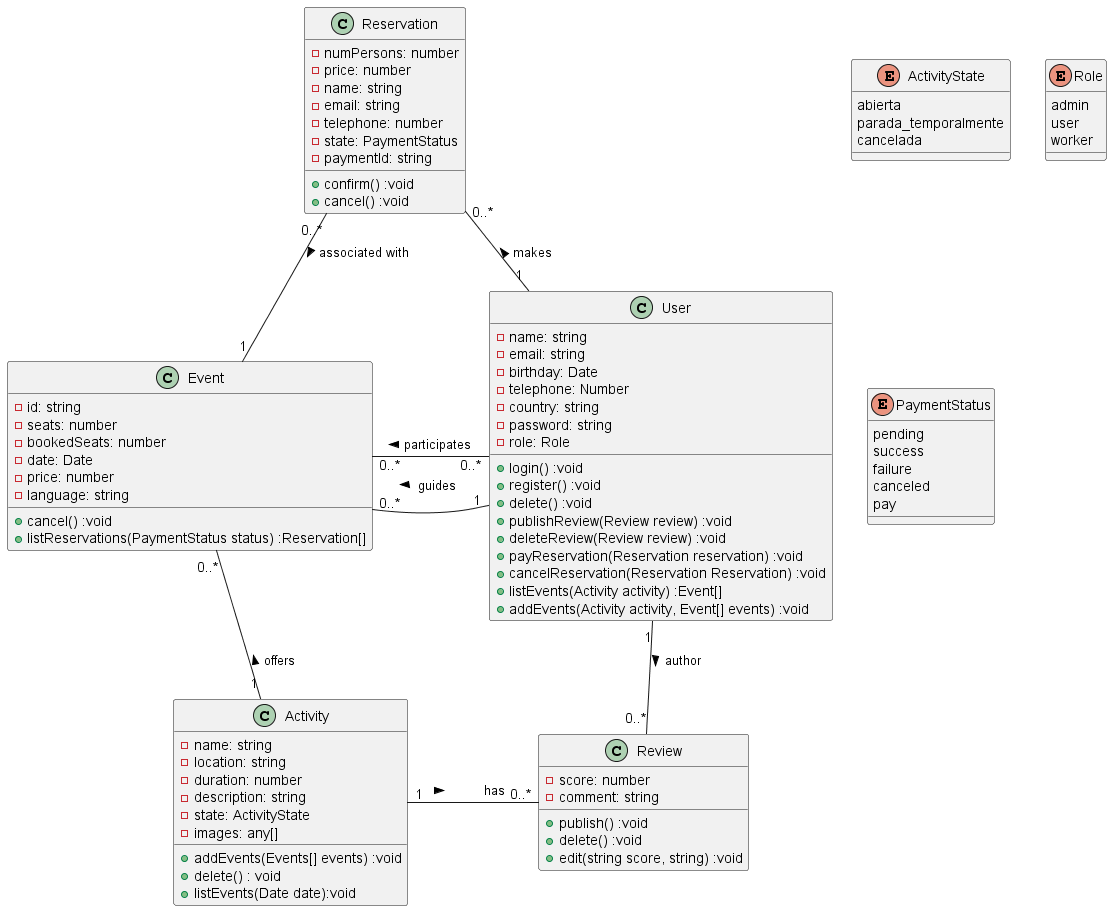
\includegraphics[width=1\textwidth]{5-AnalisisDelSistemaDeInformacion/Clases/diagrama.png}
	\caption{Diagrama de clases}
	\label{fig:mi_imagen}
\end{figure}

\subsection{Descripción de las clases}
A continuación, se detallan las clases correspondientes a los subsistemas de gestión de usuarios, actividades y reservas, cada una con una breve descripción, sus atributos y métodos propuestos.
\subsubsection{Subsistema de gestión de usuarios}
\begin{clases}
	\centering
	\begin{tabular}{|>{\raggedright\arraybackslash}p{4cm}|p{12cm}|}
		\hline
		\textbf{Nombre de la clase}   & \textbf{User}                                                                                                                                                                                                                                                          \\
		\hline
		\textbf{Descripción}          & Representa a un usuario del sistema, almacenando información personal como nombre, correo electrónico, fecha de nacimiento, y otros detalles de contacto. Los usuarios pueden tener roles diferentes que determinan sus permisos y acciones disponibles en el sistema. \\
		\hline
		\textbf{Atributos Propuestos} & \textbf{name}: string - Nombre del usuario.                                                                                                                                                                                                                            \\
		                              & \textbf{email}: string - Correo electrónico del usuario.                                                                                                                                                                                                               \\
		                              & \textbf{birthday}: Date - Fecha de nacimiento del usuario.                                                                                                                                                                                                             \\
		                              & \textbf{telephone}: Number - Número de teléfono del usuario.                                                                                                                                                                                                           \\
		                              & \textbf{country}: string - País de residencia del usuario.                                                                                                                                                                                                             \\
		                              & \textbf{password}: string - Contraseña de acceso del usuario.                                                                                                                                                                                                          \\
		                              & \textbf{role}: Role - Rol del usuario en el sistema (\textit{definido en el enum Role}).                                                                                                                                                                               \\
		\hline
		\textbf{Métodos Propuestos}   & \textbf{login(): void}                                                                                                                                                                                                                                                 \\
		                              & Permite al usuario iniciar sesión.                                                                                                                                                                                                                                     \\
		                              & \textbf{register(): void}                                                                                                                                                                                                                                              \\
		                              & Registra al usuario en el sistema.                                                                                                                                                                                                                                     \\
		                              & \textbf{delete(): void}                                                                                                                                                                                                                                                \\
		                              & Elimina la cuenta del usuario.                                                                                                                                                                                                                                         \\
		                              & \textbf{publishReview(Review review): void}                                                                                                                                                                                                                            \\
		                              & Publica una reseña.                                                                                                                                                                                                                                                    \\
		                              & \textbf{deleteReview(Review review): void}                                                                                                                                                                                                                             \\
		                              & Elimina una reseña.                                                                                                                                                                                                                                                    \\
		                              & \textbf{payReservation(Reservation reservation): void}                                                                                                                                                                                                                 \\
		                              & Realiza el pago de una reserva.                                                                                                                                                                                                                                        \\
		                              & \textbf{cancelReservation(Reservation reservation): void}                                                                                                                                                                                                              \\
		                              & Cancela una reserva.                                                                                                                                                                                                                                                   \\
		                              & \textbf{addEvents(Activity activity, Event[] events): void}                                                                                                                                                                                                            \\
		                              & Añade eventos a una actividad.                                                                                                                                                                                                                                         \\
		\hline
	\end{tabular}
	\caption{Clases - User}
\end{clases}
\subsubsection{Subsistema de gestión de actividades}
\begin{clases}
	\centering
\begin{tabular}{|>{\raggedright\arraybackslash}p{4cm}|p{12cm}|}
		\hline
		\textbf{Nombre de la clase}   & \textbf{Activity}                                                                                                                                                                                                                         \\
		\hline
		\textbf{Descripción}          & Representa una actividad ofrecida donde cada instancia incluye información detallada como ubicación, duración y una descripción. La clase gestiona los eventos asociados que pueden ocurrir en diferentes fechas o en diferentes idiomas. \\
		\hline
		\textbf{Atributos Propuestos} & \textbf{name}: string - Nombre de la actividad.                                                                                                                                                                                           \\
		                              & \textbf{location}: string - Ubicación de la actividad.                                                                                                                                                                                    \\
		                              & \textbf{duration}: number - Duración de la actividad.                                                                                                                                                                                     \\
		                              & \textbf{description}: string - Descripción de la actividad.                                                                                                                                                                               \\
		                              & \textbf{state}: ActivityState - Estado actual de la actividad (\textit{definido en el enum ActivityState}).                                                                                                                               \\
		                              & \textbf{images}: string[] - Imágenes relacionadas con la actividad.                                                                                                                                                                       \\
		\hline
		\textbf{Métodos Propuestos}   & \textbf{addEvents(Events[] events): void}                                                                                                                                                                                                 \\
		                              & Añade eventos a la actividad.                                                                                                                                                                                                             \\
		                              & \textbf{delete(): void}                                                                                                                                                                                                                   \\
		                              & Elimina la actividad.                                                                                                                                                                                                                     \\
		                              & \textbf{listEvents(Date date): void}                                                                                                                                                                                                      \\
		                              & Lista eventos según la fecha proporcionada.                                                                                                                                                                                               \\
		\hline
	\end{tabular}
	\caption{Clases - Activity}
\end{clases}

\begin{clases}
	\centering
\begin{tabular}{|>{\raggedright\arraybackslash}p{4cm}|p{12cm}|}
		\hline
		\textbf{Nombre de la clase}   & \textbf{Event}                                                                                                                                                                              \\
		\hline
		\textbf{Descripción}          & Encapsula los detalles de un evento específico asociado a una actividad. Esto incluye información sobre la capacidad de asientos, reservaciones realizadas, precio, y el idioma del evento. \\
		\hline
		\textbf{Atributos Propuestos} & \textbf{id}: string - Identificador único del evento.                                                                                                                                       \\
		                              & \textbf{seats}: number - Número total de asientos disponibles.                                                                                                                              \\
		                              & \textbf{bookedSeats}: number - Asientos reservados.                                                                                                                                         \\
		                              & \textbf{date}: Date - Fecha del evento.                                                                                                                                                     \\
		                              & \textbf{price}: number - Precio por asiento.                                                                                                                                                \\
		                              & \textbf{language}: string - Idioma en que se realiza el evento.                                                                                                                             \\
		\hline
		\textbf{Métodos Propuestos}   & \textbf{cancel(): void}                                                                                                                                                                     \\
		                              & Cancela el evento.                                                                                                                                                                          \\
		                              & \textbf{listReservations(PaymentStatus status): Reservation[]}                                                                                                                              \\
		                              & Lista las reservaciones basadas en su estado de pago.                                                                                                                                       \\

		\hline
	\end{tabular}
	\caption{Clases - Events}
\end{clases}

\begin{clases}
	\centering
\begin{tabular}{|>{\raggedright\arraybackslash}p{4cm}|p{12cm}|}
		\hline
		\textbf{Nombre de la clase}   & \textbf{Review}                                                                                                                                                                                    \\
		\hline
		\textbf{Descripción}          & Representa las reseñas que realizan los usuarios sobre las actividades. Actúa como un mecanismo para que los usuarios expresen su satisfacción o insatisfacción y mejoren la calidad de la oferta. \\
		\hline
		\textbf{Atributos Propuestos} & \textbf{score}: number - Puntuación otorgada a la actividad o evento.                                                                                                                              \\
		                              & \textbf{comment}: string - Comentario detallado sobre la experiencia.                                                                                                                              \\
		\hline
		\textbf{Métodos Propuestos}   & \textbf{publish(): void}                                                                                                                                                                           \\
		                              & Publica la reseña.                                                                                                                                                                                 \\
		                              & \textbf{delete(): void}                                                                                                                                                                            \\
		                              & Elimina la reseña.                                                                                                                                                                                 \\
		                              & \textbf{edit(string score, string comment): void}                                                                                                                                                  \\
		                              & Edita la reseña.                                                                                                                                                                                   \\
		\hline
	\end{tabular}
	\caption{Clases - Review}
\end{clases}
\subsubsection{Subsistema de gestión de reservas}
\begin{clases}
	\centering
\begin{tabular}{|>{\raggedright\arraybackslash}p{4cm}|p{12cm}|}
		\hline
		\textbf{Nombre de la clase}   & \textbf{Reservation}                                                                                                                                                                                                                                                                                                                                   \\
		\hline
		\textbf{Descripción}          & Representa las reservas hechas por los usuarios para los eventos. Cada reserva incluye detalles como el número de personas, el precio total, el estado del pago, y la identificación del evento reservado. Proporciona métodos para confirmar o cancelar reservas, y es crucial para la administración de la asistencia y los ingresos de los eventos. \\
		\hline
		\textbf{Atributos Propuestos} & \textbf{numPersons}: number - Número de personas para la reserva.                                                                                                                                                                                                                                                                                      \\
		                              & \textbf{price}: number - Precio total de la reserva.                                                                                                                                                                                                                                                                                                   \\
		                              & \textbf{name}: string - Nombre del usuario que realiza la reserva.                                                                                                                                                                                                                                                                                     \\
		                              & \textbf{email}: string - Correo electrónico del usuario que realiza la reserva.                                                                                                                                                                                                                                                                        \\
		                              & \textbf{telephone}: number - Número de teléfono del usuario que realiza la reserva.                                                                                                                                                                                                                                                                    \\
		                              & \textbf{state}: PaymentStatus - Estado del pago de la reserva (pendiente, éxito, fallo, cancelado, pago).                                                                                                                                                                                                                                              \\
		                              & \textbf{paymentId}: string - Identificador único del pago.                                                                                                                                                                                                                                                                                             \\
		\hline
		\textbf{Métodos Propuestos}   & \textbf{confirm(): void}                                                                                                                                                                                                                                                                                                                               \\
		                              & Confirma la reserva.                                                                                                                                                                                                                                                                                                                                   \\
		                              & \textbf{cancel(): void}                                                                                                                                                                                                                                                                                                                                \\
		                              & Cancela la reserva.                                                                                                                                                                                                                                                                                                                                    \\
		\hline
	\end{tabular}
	\caption{Clases - Reservation}
\end{clases}
\section{Definición de interfaces de usuario}
\subsection{Descripción de la interfaz }
En este apartado se mostrarán los bocetos que se han realizado para la interfaz de usuario de este proyecto. Las vistas sufren ligeras modificaciones dependiendo del rol que tenga el usuario, si está registrado o no, así como el dispositivo que se esté usando. Se han identificado las siguientes ventanas.
\subsubsection{Inicio}
La vista “Inicio” será aquella que se vea nada más acceder a la aplicación. En ella se pondrá observar la lista de actividades más populares así como un botón para poder ir directamente a la búsqueda de actividades.
\begin{figure}[H]
	\centering
	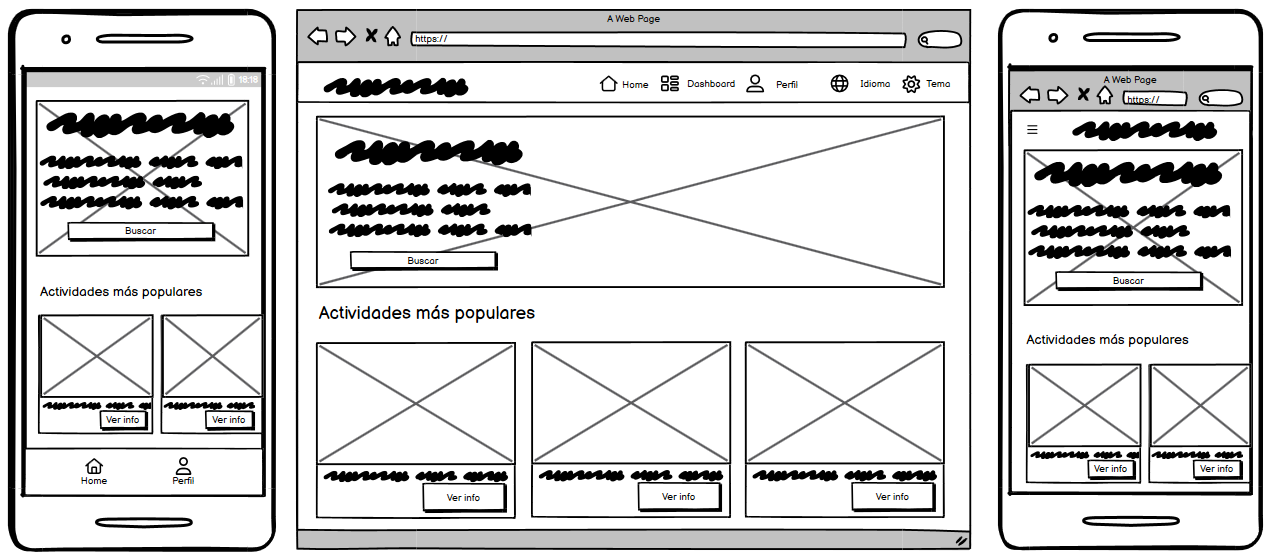
\includegraphics[width=0.8\textwidth]{5-AnalisisDelSistemaDeInformacion/InterfacesDeUsuario/Inicio/inicio-admin.png}
	\caption{Inicio - Vista Administrador }
\end{figure}

\begin{figure}[H]
	\centering
	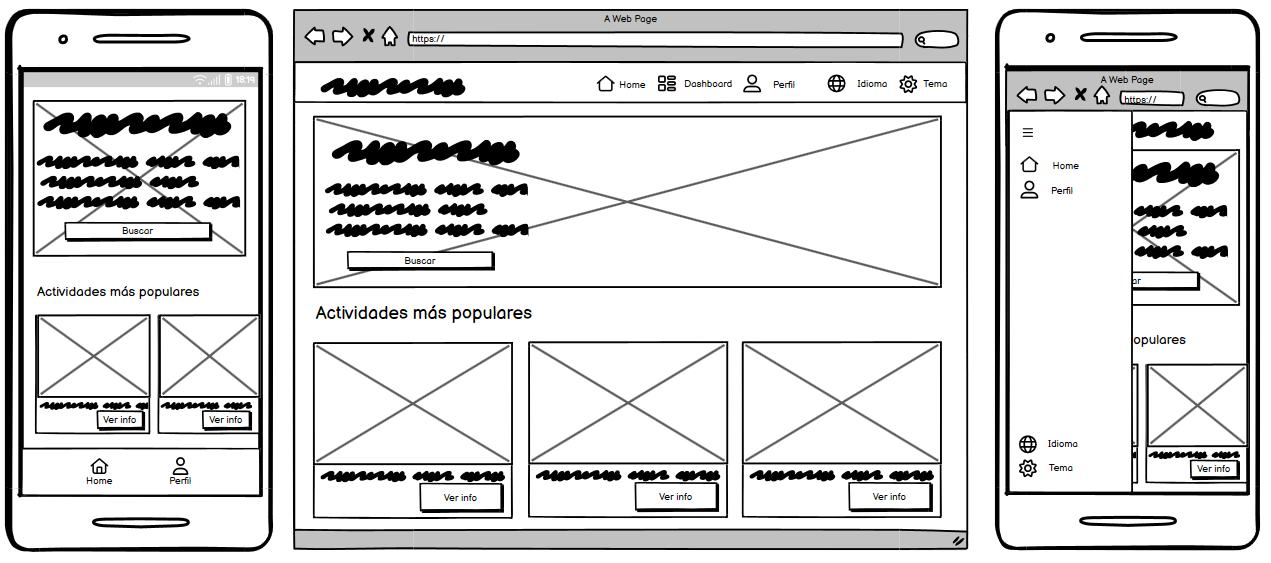
\includegraphics[width=0.8\textwidth]{5-AnalisisDelSistemaDeInformacion/InterfacesDeUsuario/Inicio/inicio-admin-menu.png}
	\caption{Inicio - Vista Administrador (Menú desplegado)}
\end{figure}

\begin{figure}[H]
	\centering
	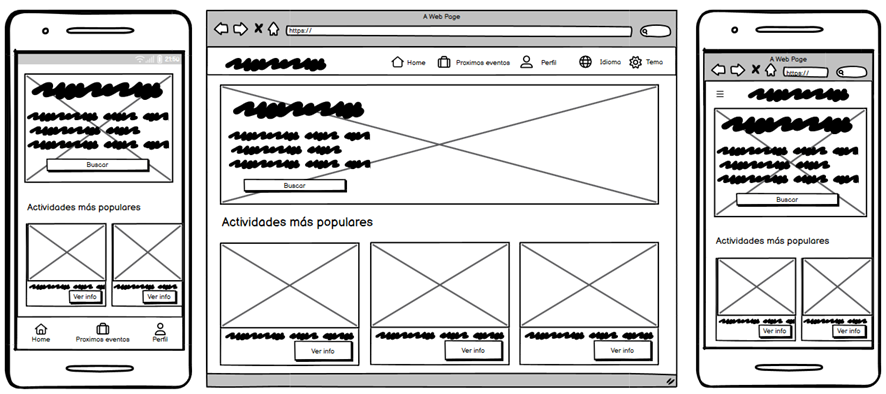
\includegraphics[width=0.8\textwidth]{5-AnalisisDelSistemaDeInformacion/InterfacesDeUsuario/Inicio/inicio-guia.png}
	\caption{Inicio - Vista Guía }
\end{figure}

\begin{figure}[H]
	\centering
	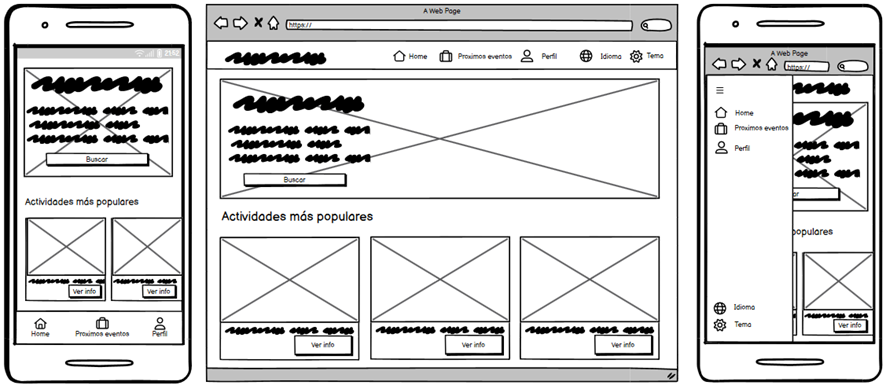
\includegraphics[width=0.8\textwidth]{5-AnalisisDelSistemaDeInformacion/InterfacesDeUsuario/Inicio/inicio-guia-menu.png}
	\caption{Inicio - Vista Guía (Menú desplegado)}
\end{figure}

\begin{figure}[H]
	\centering
	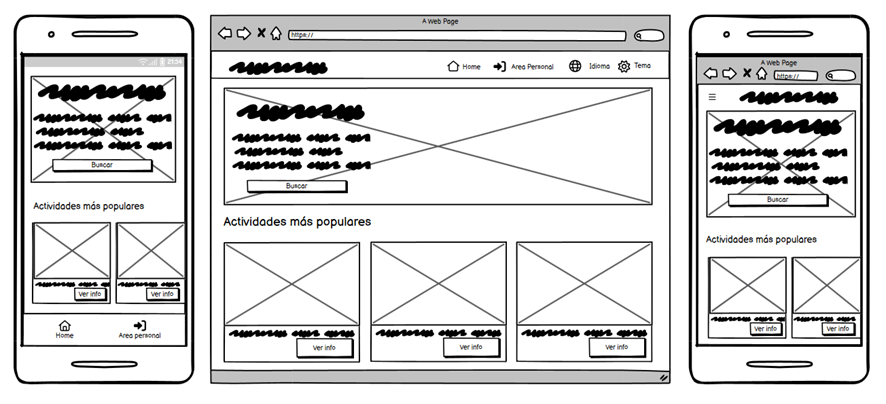
\includegraphics[width=0.8\textwidth]{5-AnalisisDelSistemaDeInformacion/InterfacesDeUsuario/Inicio/inicio-no-identificado.png}
	\caption{Inicio - Vista Usuario no identificado }
\end{figure}

\begin{figure}[H]
	\centering
	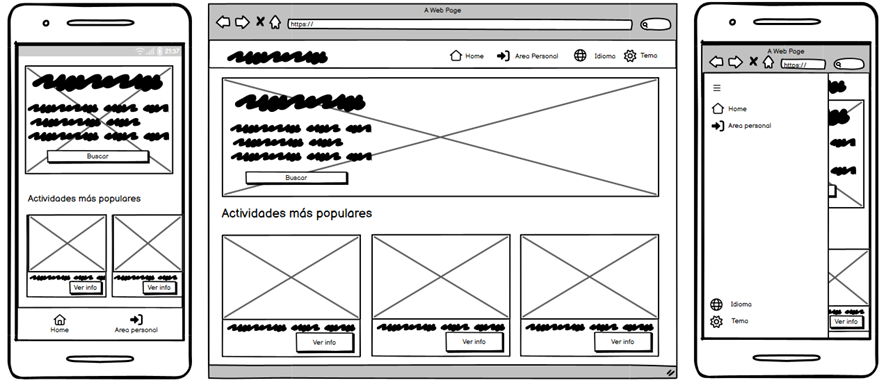
\includegraphics[width=0.8\textwidth]{5-AnalisisDelSistemaDeInformacion/InterfacesDeUsuario/Inicio/inicio-no-identificado-menu.png}
	\caption{Inicio - Vista Usuario no identificado (Menú desplegado)}
\end{figure}

\begin{figure}[H]
	\centering
	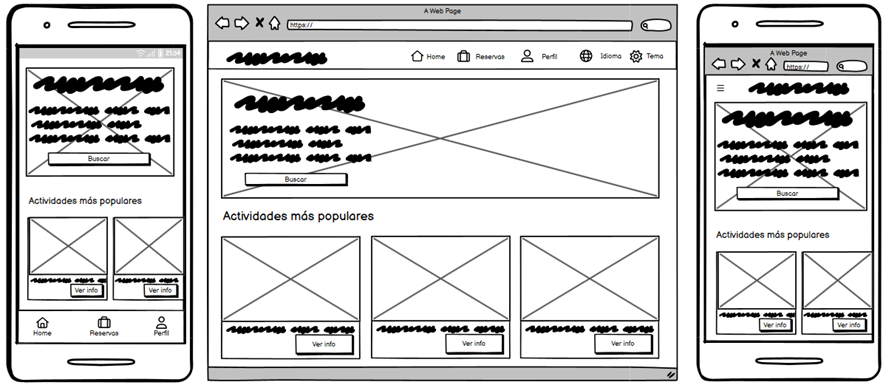
\includegraphics[width=0.8\textwidth]{5-AnalisisDelSistemaDeInformacion/InterfacesDeUsuario/Inicio/inicio-turista.png}
	\caption{Inicio - Vista Turista }
\end{figure}

\begin{figure}[H]
	\centering
	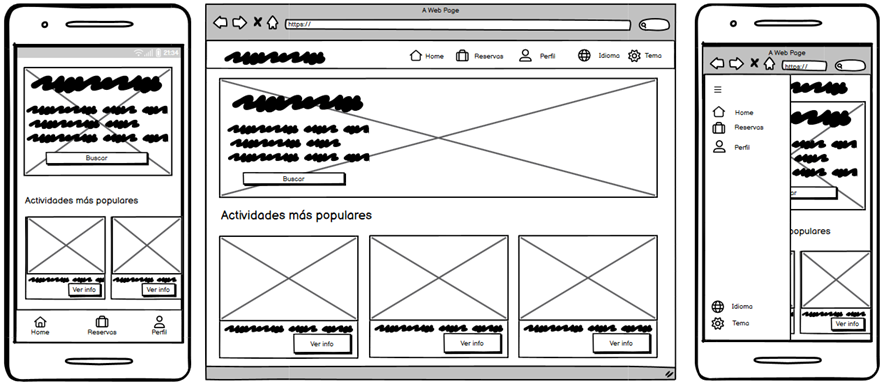
\includegraphics[width=0.8\textwidth]{5-AnalisisDelSistemaDeInformacion/InterfacesDeUsuario/Inicio/inicio-turista-menu.png}
	\caption{Inicio - Vista Turista (Menú desplegado)}
\end{figure}

\subsubsection{Inicio de sesión}
La vista “Inicio de sesión” será aquella vista que se enseñará cuando el usuario quiera identificarse en la aplicación.
En esta vista el usuario podrá introducir su correo electrónico y contraseña para poder acceder a la aplicación.
\begin{figure}[H]
	\centering
	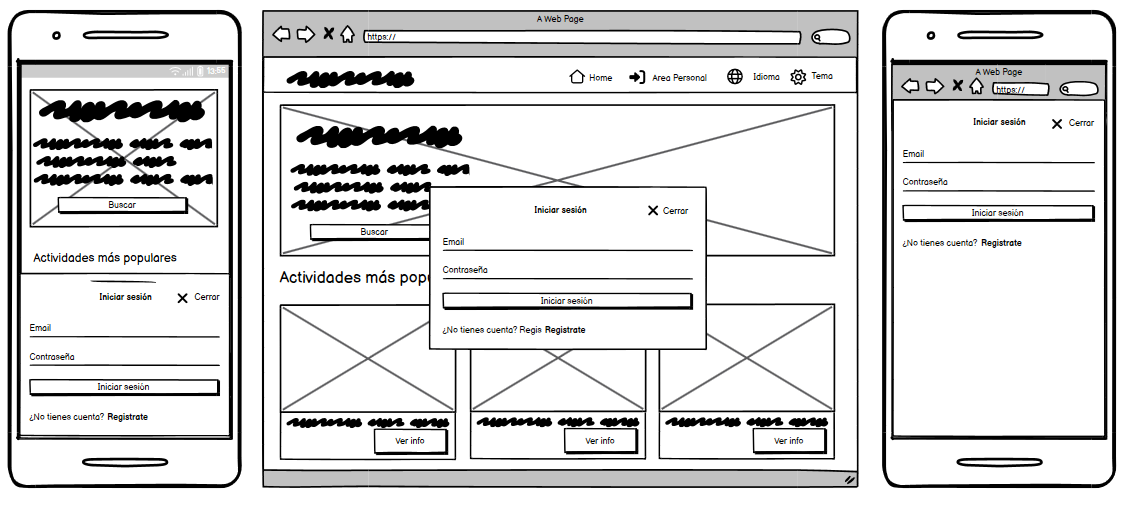
\includegraphics[width=0.8\linewidth]{5-AnalisisDelSistemaDeInformacion/InterfacesDeUsuario/InicioDeSesion/inicioDeSesion.png}
	\caption{Inicio de sesión}
\end{figure}
\subsubsection{Registro}
La vista “Registro” será aquella vista que se enseñará cuando el usuario quiera registrarse en la aplicación.
En esta vista el usuario deberá introducir sus datos personales y una contraseña.
\begin{figure}[H]
	\centering
	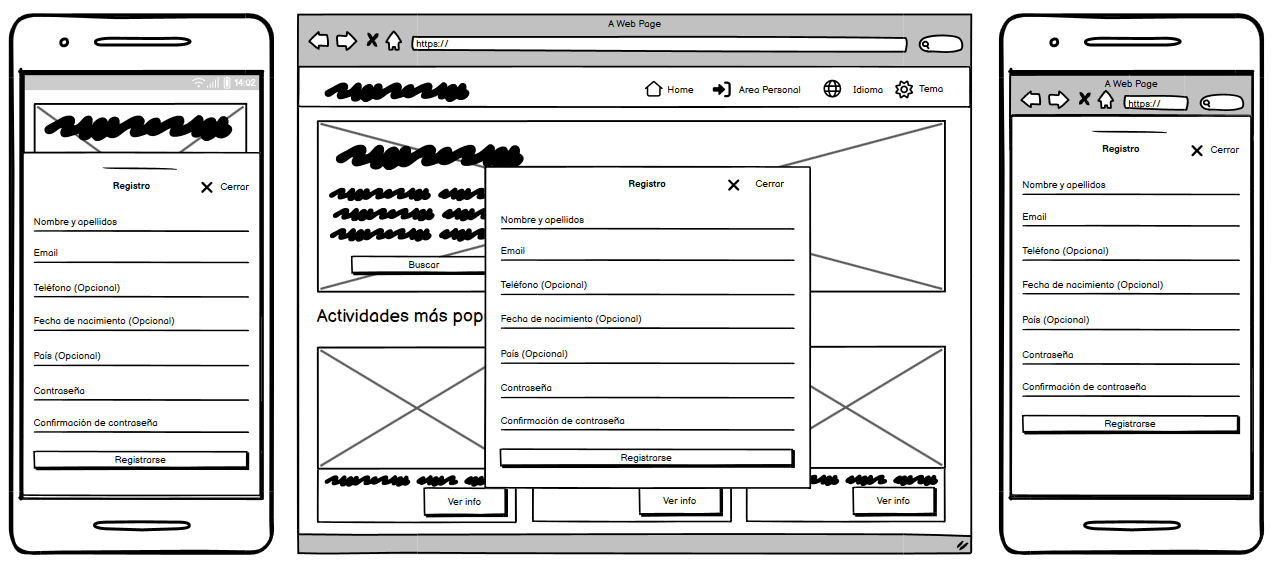
\includegraphics[width=0.8\linewidth]{5-AnalisisDelSistemaDeInformacion/InterfacesDeUsuario/Registro/registro.png}
	\caption{Registro}
\end{figure}
\subsubsection{Buscar actividades}
La vista “Buscar actividades” será aquella vista que se enseñará cuando el usuario quiera hacer una búsqueda de las actividades. En esta búsqueda el usuario podrá aplicar filtros y ordenar los resultados según el criterio que más le convenga.
\begin{figure}[H]
	\centering
	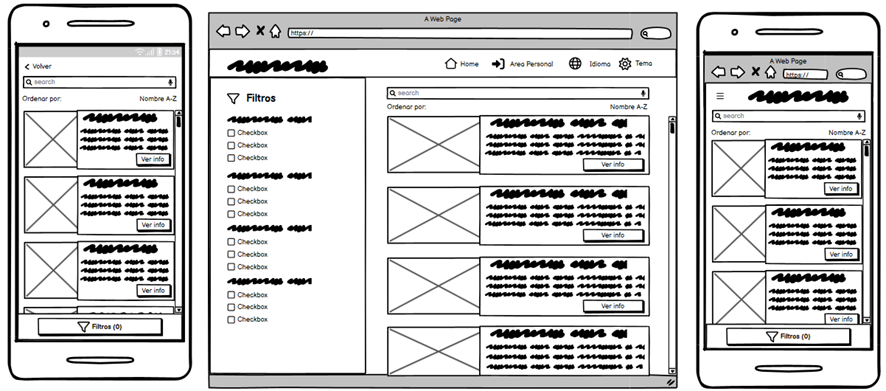
\includegraphics[width=0.8\linewidth]{5-AnalisisDelSistemaDeInformacion/InterfacesDeUsuario/BuscarActividades/buscar-standar.png}
	\caption{Buscar Actividades}
\end{figure}

\begin{figure}[H]
	\centering
	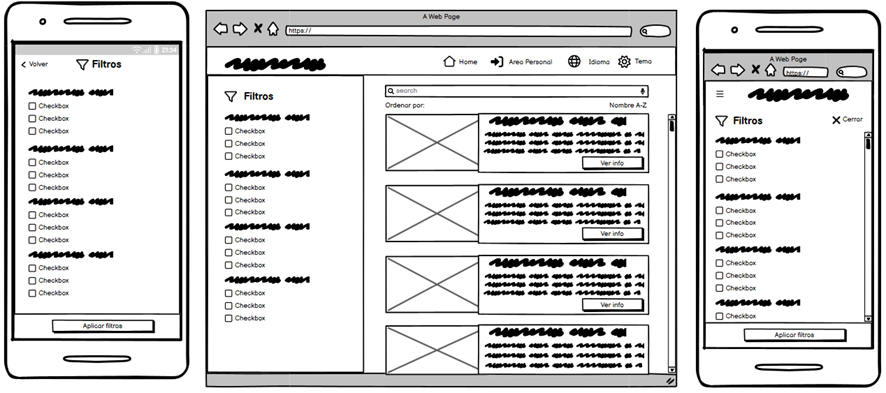
\includegraphics[width=0.8\linewidth]{5-AnalisisDelSistemaDeInformacion/InterfacesDeUsuario/BuscarActividades/buscar-standar-aplicando-filtros.png}
	\caption{Buscar Actividades - Aplicar Filtros}
\end{figure}

\begin{figure}[H]
	\centering
	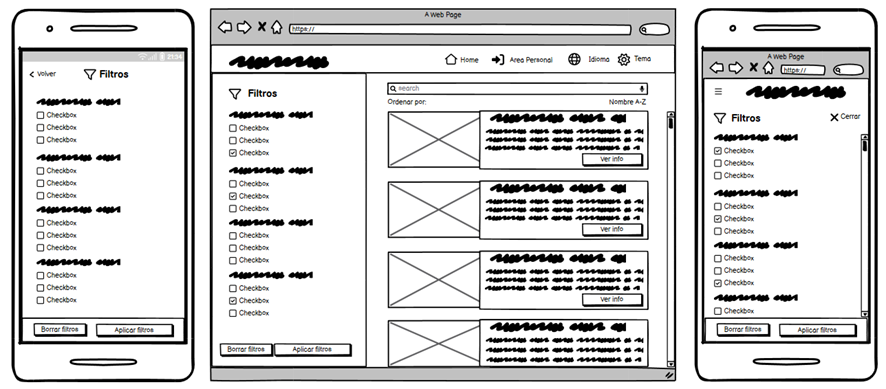
\includegraphics[width=0.8\linewidth]{5-AnalisisDelSistemaDeInformacion/InterfacesDeUsuario/BuscarActividades/buscar-standar-borrar-filtros.png}
	\caption{Buscar Actividades - Borrar Filtros}
\end{figure}

\begin{figure}[H]
	\centering
	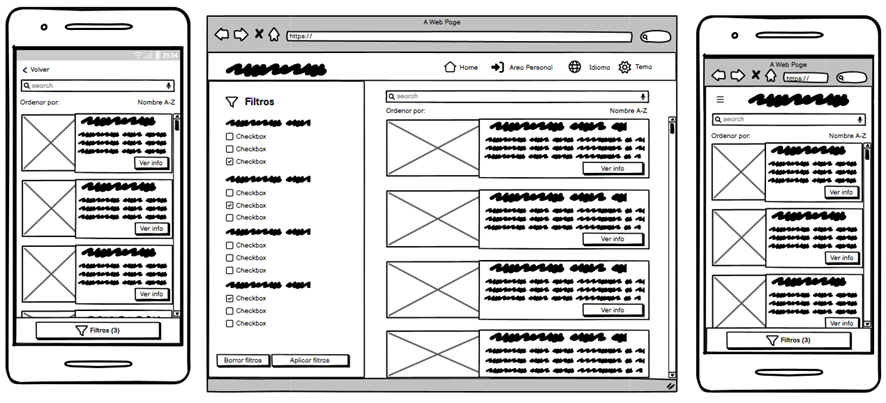
\includegraphics[width=0.8\linewidth]{5-AnalisisDelSistemaDeInformacion/InterfacesDeUsuario/BuscarActividades/buscar-standar-con-filtros.png}
	\caption{Buscar Actividades - Con Filtros}
\end{figure}


\subsubsection{Detalles de actividad}
La vista “Detalles de actividad” será aquella vista que se enseñará cuando el usuario quiera ver la información asociada a la actividad. En esta vista el usuario también podrá ver las valoraciones y la disponibilidad en caso de que la actividad tenga eventos con plazas disponibles.
\begin{figure}[H]
	\centering
	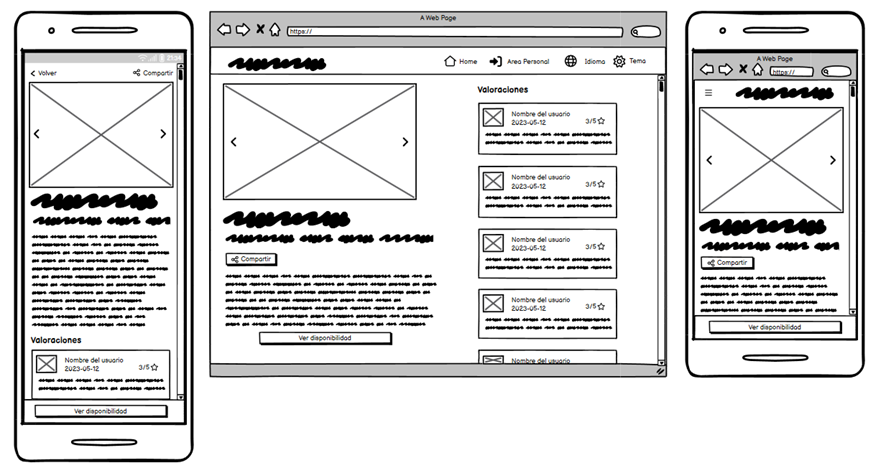
\includegraphics[width=0.8\textwidth]{5-AnalisisDelSistemaDeInformacion/InterfacesDeUsuario/Detalles de actividad/detalles-estandar.png}
	\caption{Detalles de actividad}
\end{figure}

\begin{figure}[H]
	\centering
	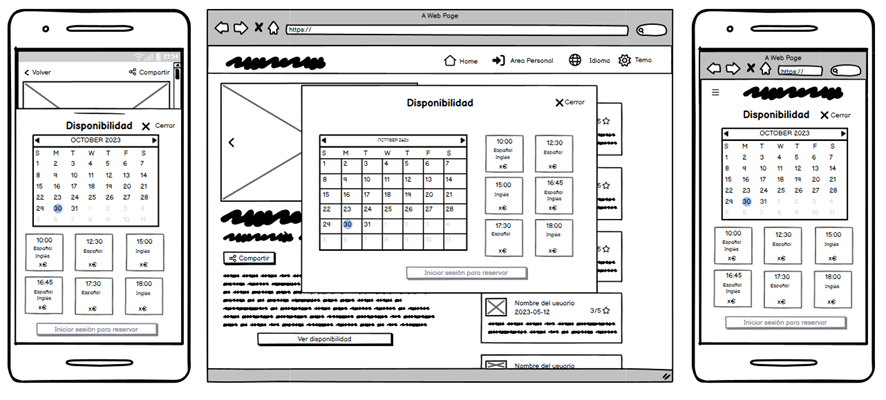
\includegraphics[width=0.8\textwidth]{5-AnalisisDelSistemaDeInformacion/InterfacesDeUsuario/Detalles de actividad/detalles-estandar-disponibilidad.png}
	\caption{Detalles de actividad - Disponibilidad}
\end{figure}
\subsubsection{Realizar reserva}
La vista “Realizar reserva” será aquella vista que se enseñará cuando el usuario quiera empiece el proceso de compra. En esta vista el usuario pasará por distintos pasos donde deberá introducir datos personales y datos bancarios para realizar la reserva.
\begin{figure}[H]
	\centering
	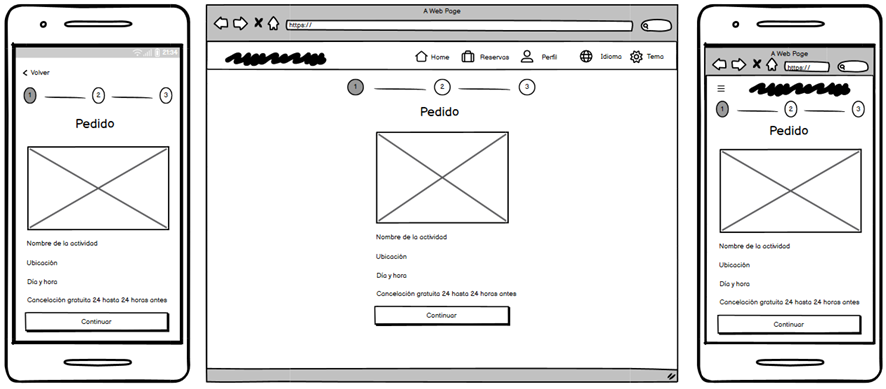
\includegraphics[width=0.8\linewidth]{5-AnalisisDelSistemaDeInformacion/InterfacesDeUsuario/Reservar/reservar-paso1.png}
	\caption{Realizar reserva - Paso 1: Selección de opciones}
	\label{fig:paso1}
\end{figure}

\begin{figure}[H]
	\centering
	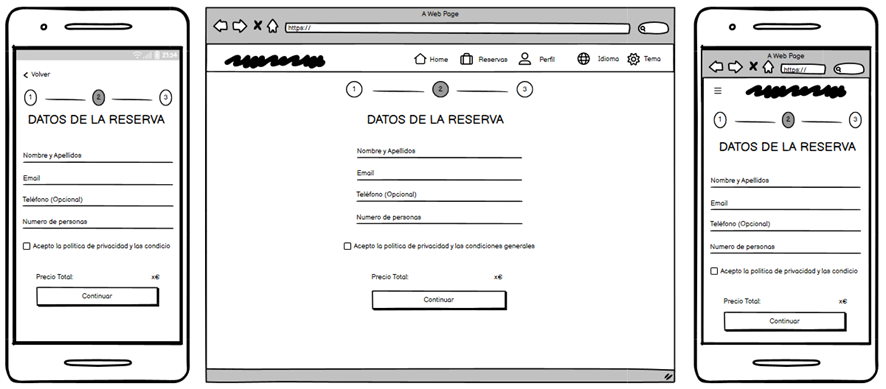
\includegraphics[width=0.8\linewidth]{5-AnalisisDelSistemaDeInformacion/InterfacesDeUsuario/Reservar/reservar-paso2-personales.png}
	\caption{Realizar reserva - Paso 2: Información personal}
	\label{fig:paso2-personales}
\end{figure}

\begin{figure}[H]
	\centering
	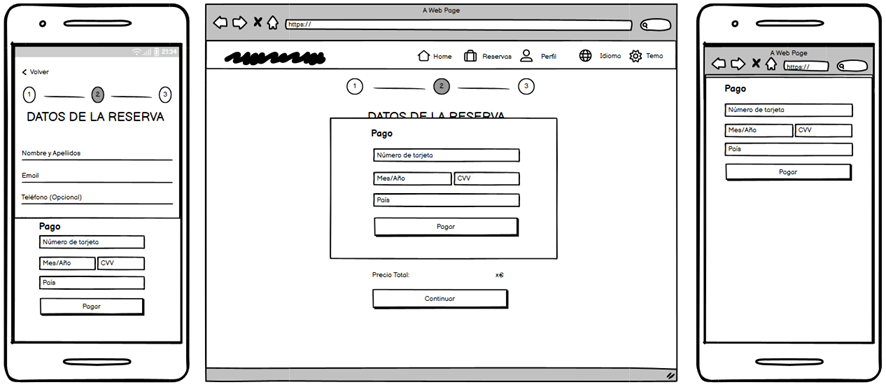
\includegraphics[width=0.8\linewidth]{5-AnalisisDelSistemaDeInformacion/InterfacesDeUsuario/Reservar/reservar-paso2-bancarios.png}
	\caption{Realizar reserva - Paso 2: Información bancaria}
	\label{fig:paso2-bancarios}
\end{figure}

\begin{figure}[H]
	\centering
	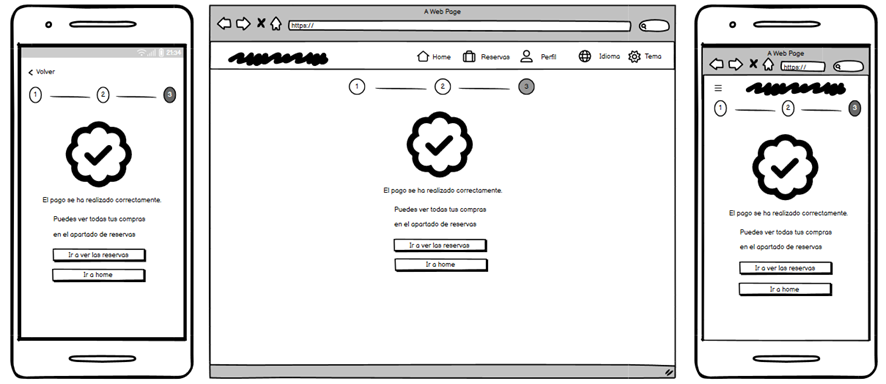
\includegraphics[width=0.8\linewidth]{5-AnalisisDelSistemaDeInformacion/InterfacesDeUsuario/Reservar/reservar-paso3.png}
	\caption{Realizar reserva - Paso 3: Confirmación}
	\label{fig:paso3}
\end{figure}
\subsubsection{Lista de reservas}
En esta vista “Lista de reservas” el usuario podrá ver todas las reservas realizadas agrupadas por rangos de fechas próximas.
\begin{figure}[H]
	\centering
	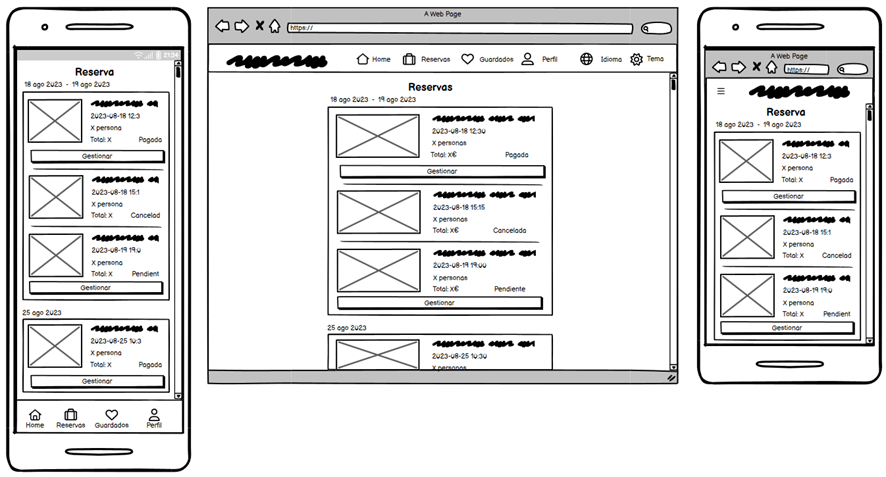
\includegraphics[width=0.8\linewidth]{5-AnalisisDelSistemaDeInformacion/InterfacesDeUsuario/Lista de reservas/lista.png}
	\caption{Lista de reservas}
\end{figure}
\subsubsection*{Gestión de reserva}
En esta vista “Gestión de reserva” el usuario podrá ver la información asociada a la reserva, añadir una reseña si ha completado la reserva, así como cancelarla si lo desea.
\begin{figure}[H]
	\centering
	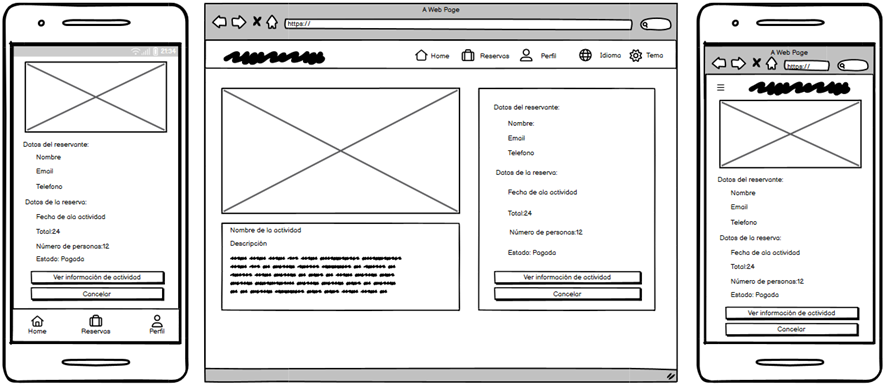
\includegraphics[width=0.8\textwidth]{5-AnalisisDelSistemaDeInformacion/InterfacesDeUsuario/Detalles de reserva/detalles.png}
	\caption{Gestión de reserva}
\end{figure}
\subsubsection{Perfil}
En esta vista “Perfil” el usuario podrá ver todos sus datos personales, asi como gestionar su cuenta, ya sea para cambiar la contraseña o para cancelar la cuenta.
\begin{figure}[H]
	\centering
	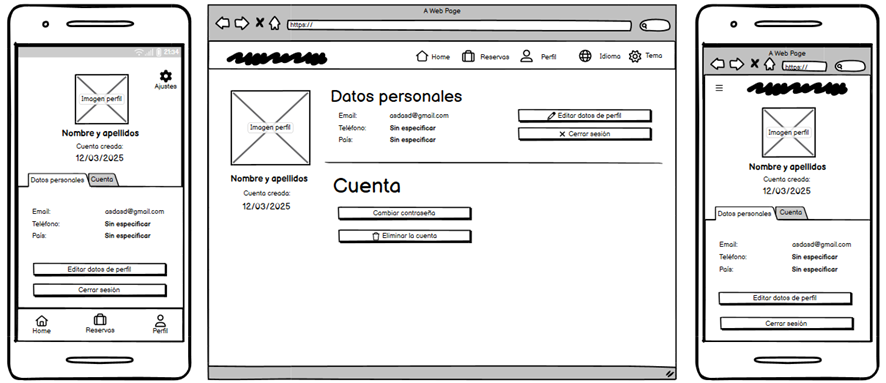
\includegraphics[width=0.8\linewidth]{5-AnalisisDelSistemaDeInformacion/InterfacesDeUsuario/Perfil/perfil-personales.png}
	\caption{Perfil - Datos Personales}
\end{figure}

\begin{figure}[H]
	\centering
	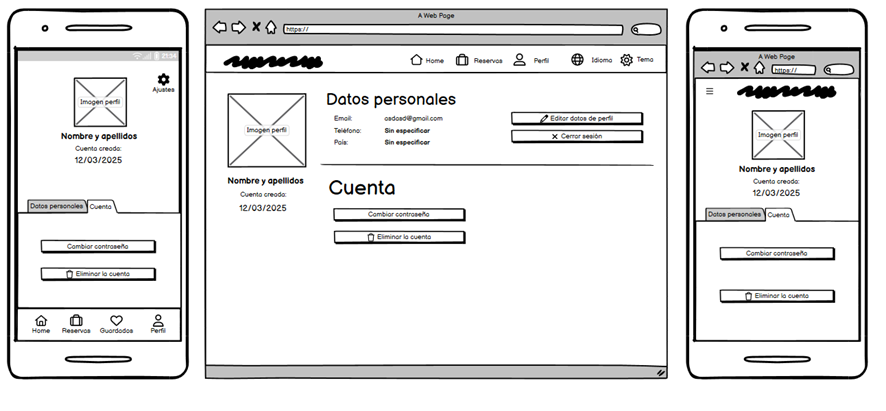
\includegraphics[width=0.8\linewidth]{5-AnalisisDelSistemaDeInformacion/InterfacesDeUsuario/Perfil/perfil-cuenta.png}
	\caption{Perfil - Cuenta}
\end{figure}

\begin{figure}[H]
	\centering
	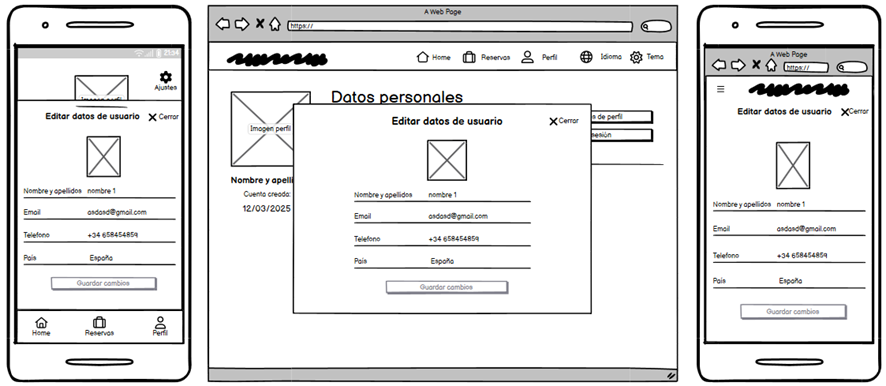
\includegraphics[width=0.8\linewidth]{5-AnalisisDelSistemaDeInformacion/InterfacesDeUsuario/Perfil/perfil-cambio-personales.png}
	\caption{Perfil - Cambio de Datos Personales}
\end{figure}

\begin{figure}[H]
	\centering
	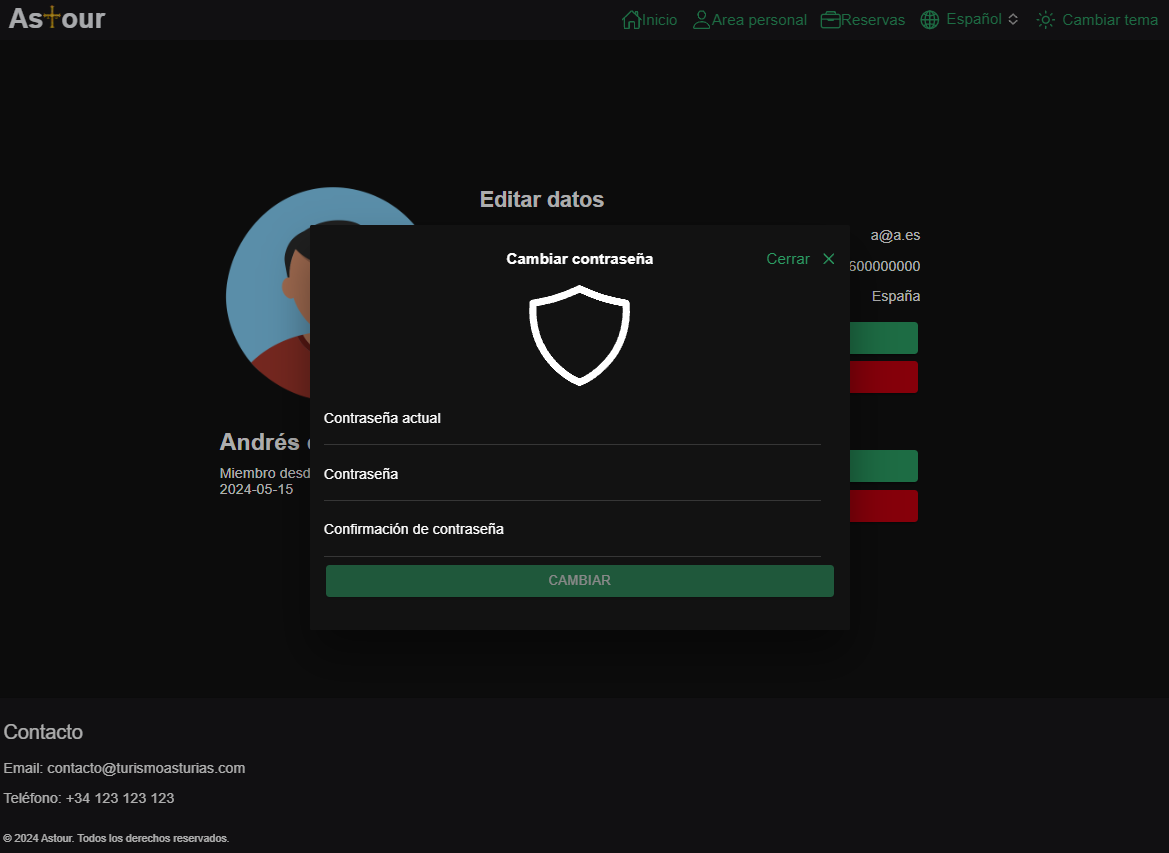
\includegraphics[width=0.8\linewidth]{5-AnalisisDelSistemaDeInformacion/InterfacesDeUsuario/Perfil/perfil-cambio-contraseña.png}
	\caption{Perfil - Cambio de Contraseña}
\end{figure}
\subsubsection{Dashboard}
En esta vista “Dashboard” el usuario registrado como administrador podrá ver los datos estadísticos de la aplicación, así como gestionar las actividades y los usuarios.
\begin{figure}[H]
	\centering
	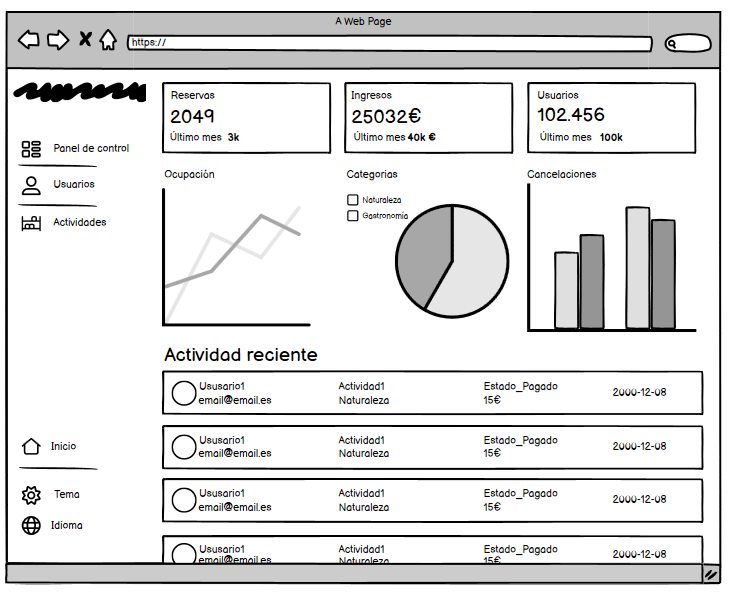
\includegraphics[width=0.8\textwidth]{5-AnalisisDelSistemaDeInformacion/InterfacesDeUsuario/Dashboard/panel de control.png}
	\caption{Dashboard - Panel de control}
\end{figure}


En el apartado “Usuarios” de la vista “Dashboard” se muestra una lista de los usuarios registrados en el sistema.
En la tabla se muestra el nombre, correo electrónico, el rol y las reservas realizadas de cada usuario.
Además, se incluye un botón para ver los detalles de cada usuario que nos llevará a la vista “Detalles de usuario” .

\begin{figure}[H]
	\centering
	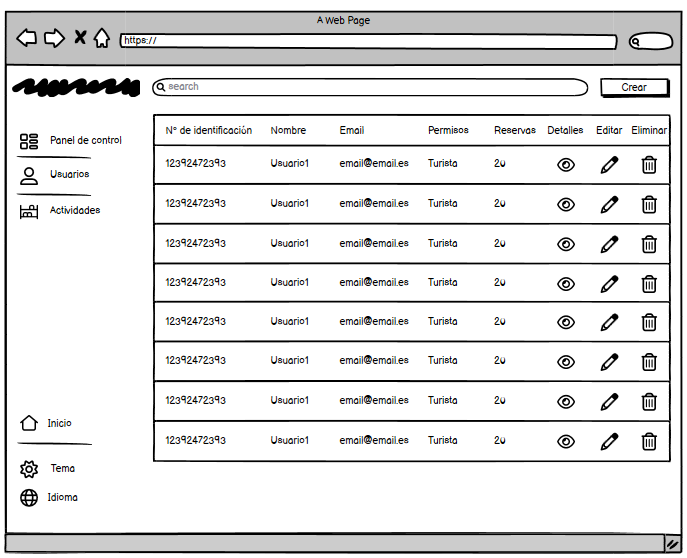
\includegraphics[width=0.8\textwidth]{5-AnalisisDelSistemaDeInformacion/InterfacesDeUsuario/Dashboard/lista usuarios.png}
	\caption{Dashboard - Lista de usuarios}
\end{figure}

\begin{figure}[H]
	\centering
	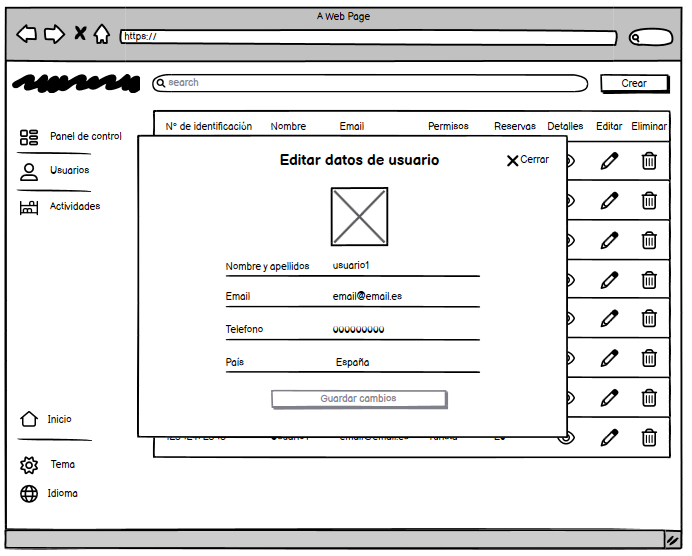
\includegraphics[width=0.8\textwidth]{5-AnalisisDelSistemaDeInformacion/InterfacesDeUsuario/Dashboard/lista usuarios edit.png}
	\caption{Dashboard - Editar usuario}
\end{figure}

En el apartado “Actividades” de la vista “Dashboard” se muestra una lista de las actividades registradas en el sistema.
En la tabla se muestra el nombre, fecha de inicio, fecha de fin, lugar, descripción y el estado de cada actividad.
En caso de querer ver los eventos de una actividad, se puede hacer clic en la opción del menú lateral “Mostrar eventos” .

\begin{figure}[H]
	\centering
	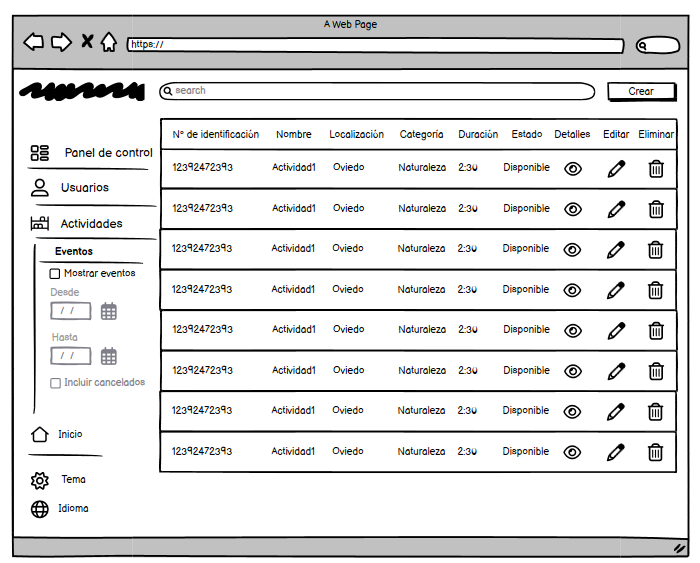
\includegraphics[width=0.8\textwidth]{5-AnalisisDelSistemaDeInformacion/InterfacesDeUsuario/Dashboard/lista de actividades.png}
	\caption{Dashboard - Lista de actividades}
\end{figure}

\begin{figure}[H]
	\centering
	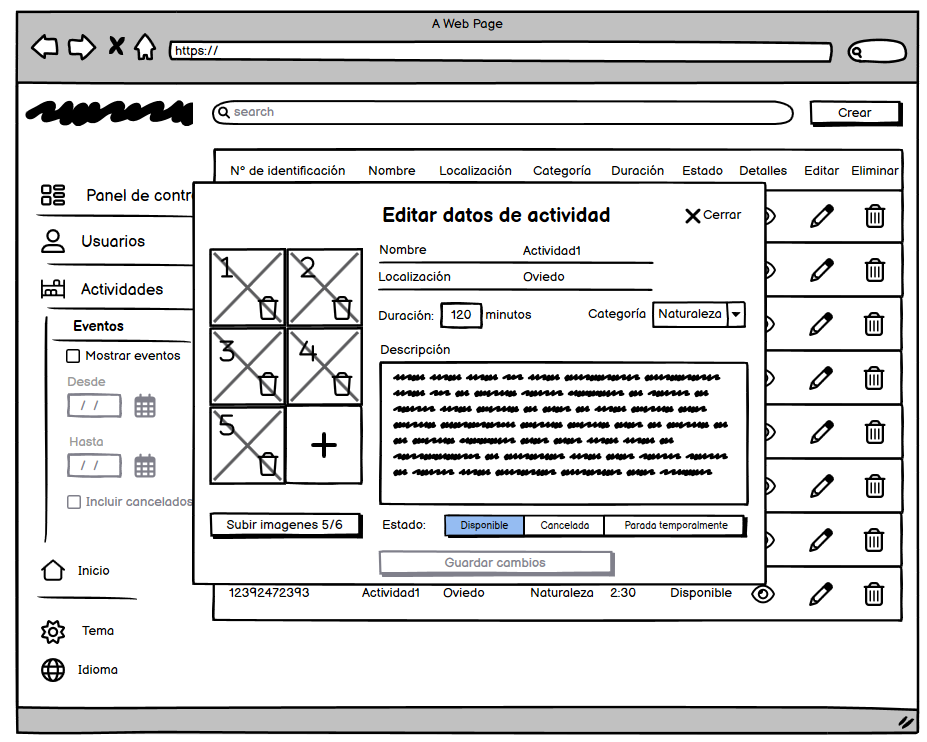
\includegraphics[width=0.8\textwidth]{5-AnalisisDelSistemaDeInformacion/InterfacesDeUsuario/Dashboard/lista de actividades edit.png}
	\caption{Dashboard - Lista de actividades}
\end{figure}

\begin{figure}[H]
	\centering
	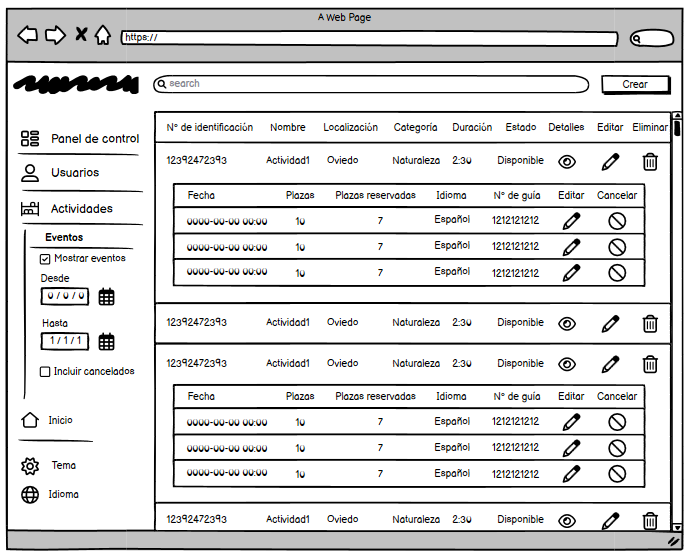
\includegraphics[width=0.8\textwidth]{5-AnalisisDelSistemaDeInformacion/InterfacesDeUsuario/Dashboard/lista eventos.png}
	\caption{Dashboard - Lista de actividades con eventos}
\end{figure}

\begin{figure}[H]
	\centering
	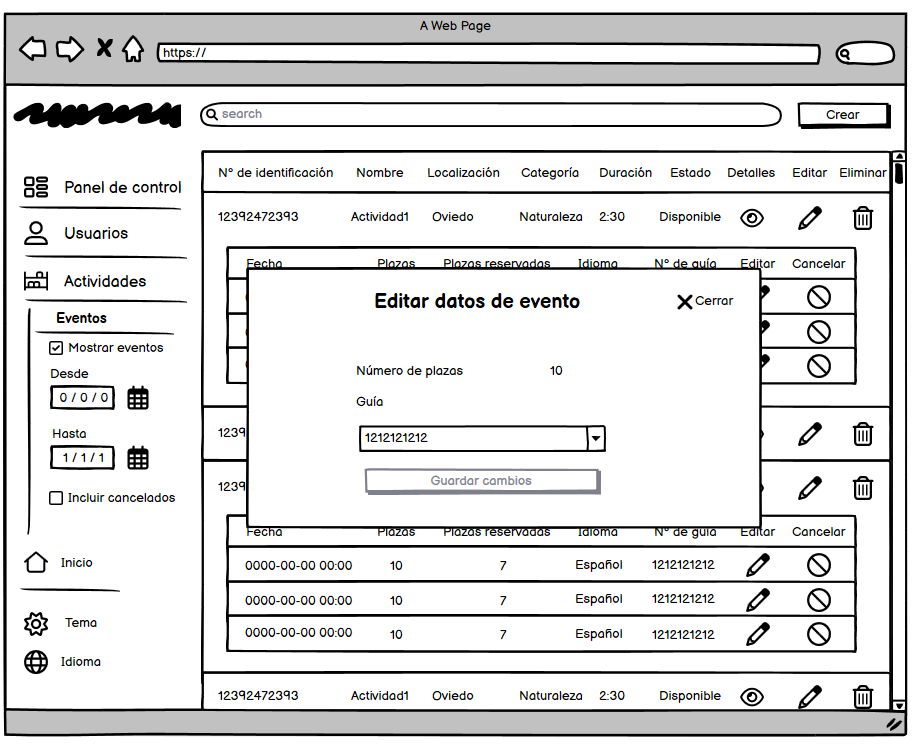
\includegraphics[width=0.8\textwidth]{5-AnalisisDelSistemaDeInformacion/InterfacesDeUsuario/Dashboard/lista eventos edit.png}
	\caption{Dashboard - Editar evento}
\end{figure}

\subsubsection*{Detalles de usuario}
En la vista “Detalles de usuario” se muestra la información personal de un usuario, así como las reservas realizadas por el mismo.
Además, se incluye un botón para editar los datos del usuario y otro para editar una reserva.

\begin{figure}[H]
	\centering
	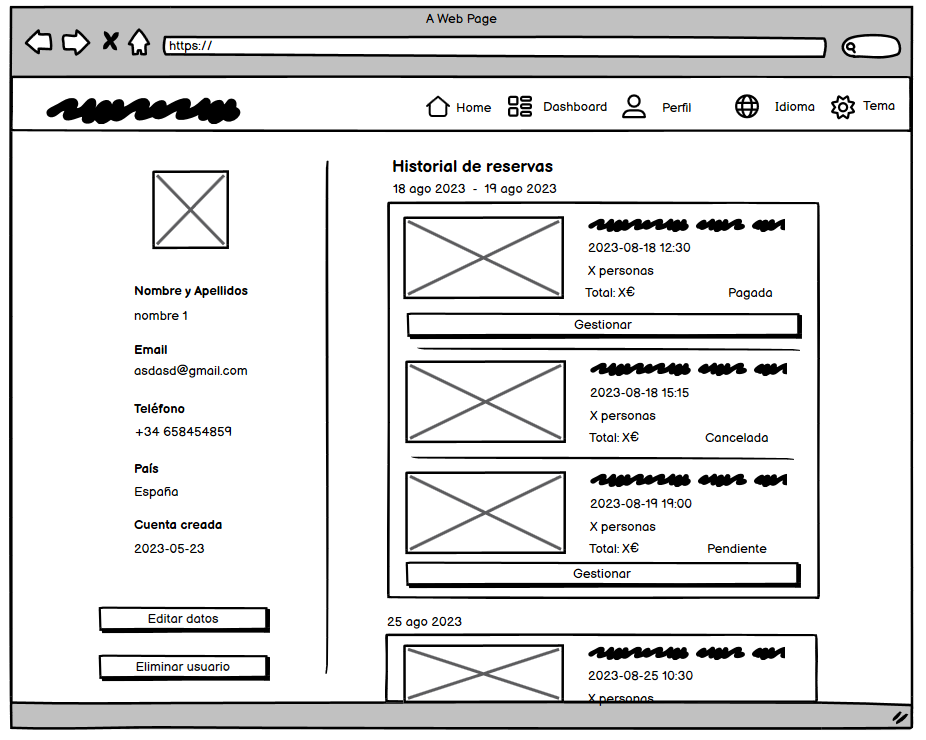
\includegraphics[width=0.8\textwidth]{5-AnalisisDelSistemaDeInformacion/InterfacesDeUsuario/Dashboard/detalles usuario.png}
	\caption{Detalles de usuario}
\end{figure}

\begin{figure}[H]
	\centering
	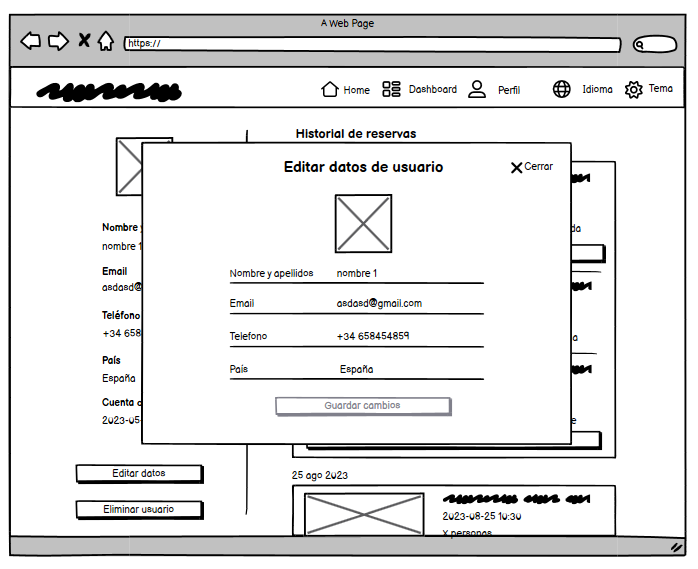
\includegraphics[width=0.8\textwidth]{5-AnalisisDelSistemaDeInformacion/InterfacesDeUsuario/Dashboard/detalles usuario editar datos.png}
	\caption{Detalles de usuario - Editar datos}
\end{figure}

\begin{figure}[H]
	\centering
	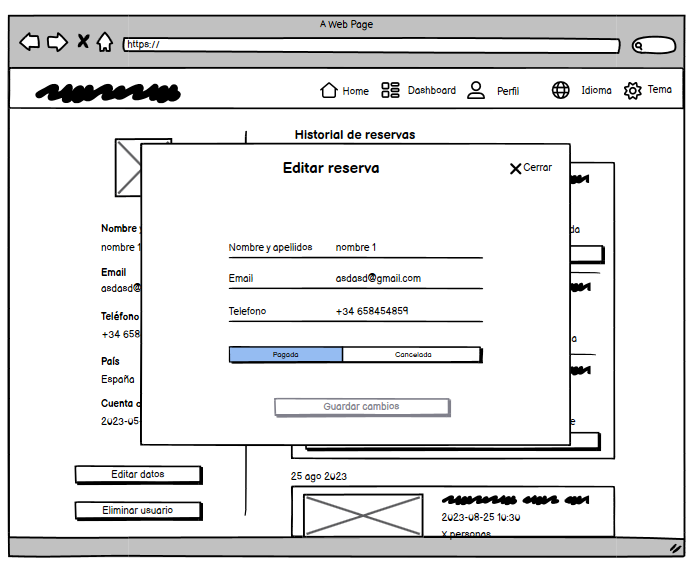
\includegraphics[width=0.8\textwidth]{5-AnalisisDelSistemaDeInformacion/InterfacesDeUsuario/Dashboard/detalles usuario editar reserva.png}
	\caption{Detalles de usuario - Editar reserva}
\end{figure}

\subsubsection{Eventos próximos}
En esta vista “Eventos próximos” el usuario registrado como guía podrá ver los eventos que tiene próximamente planificados, así como información de contacto de los turistas que han reservado.
\begin{figure}[H]
	\centering
	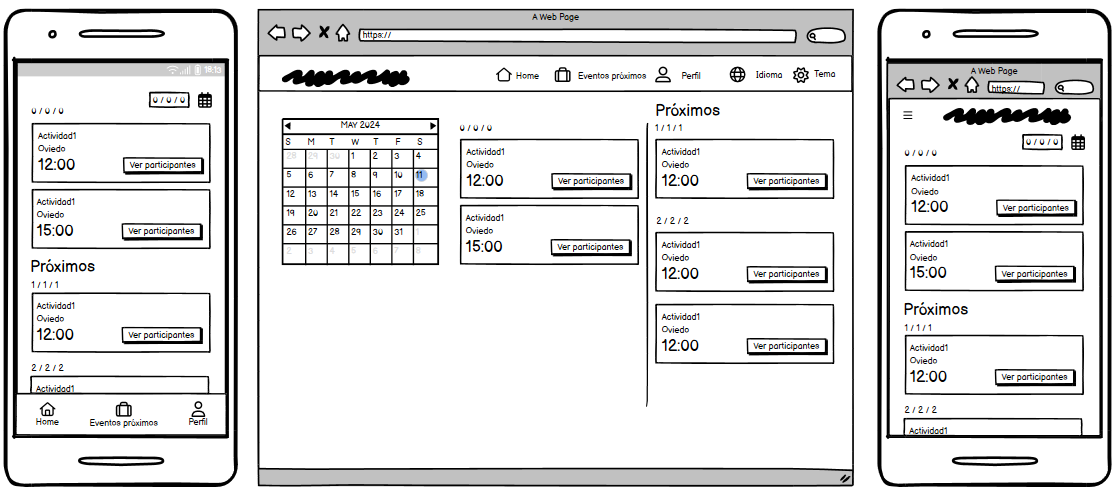
\includegraphics[width=0.8\textwidth]{5-AnalisisDelSistemaDeInformacion/InterfacesDeUsuario/EventosProximos/eventos proximos.png}
	\caption{Eventos próximos}
\end{figure}

\begin{figure}[H]
	\centering
	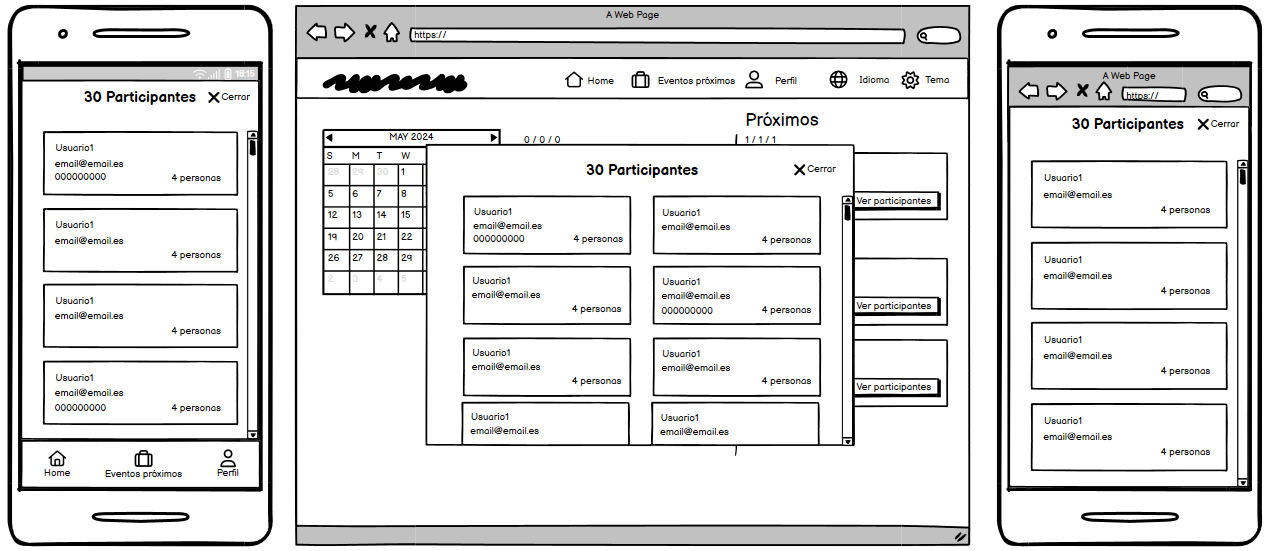
\includegraphics[width=0.8\textwidth]{5-AnalisisDelSistemaDeInformacion/InterfacesDeUsuario/EventosProximos/eventos proximos participantes.png}
	\caption{Eventos próximos - Participantes}
\end{figure}

\subsection{Descripción del comportamiento de la interfaz}
\subsubsection{Diagrama de navegabilidad}
A continuación se presenta el diagrama de navegabilidad, que ilustra las relaciones y transiciones entre las diferentes páginas y componentes de la interfaz
\begin{figure}[H]
	\centering
	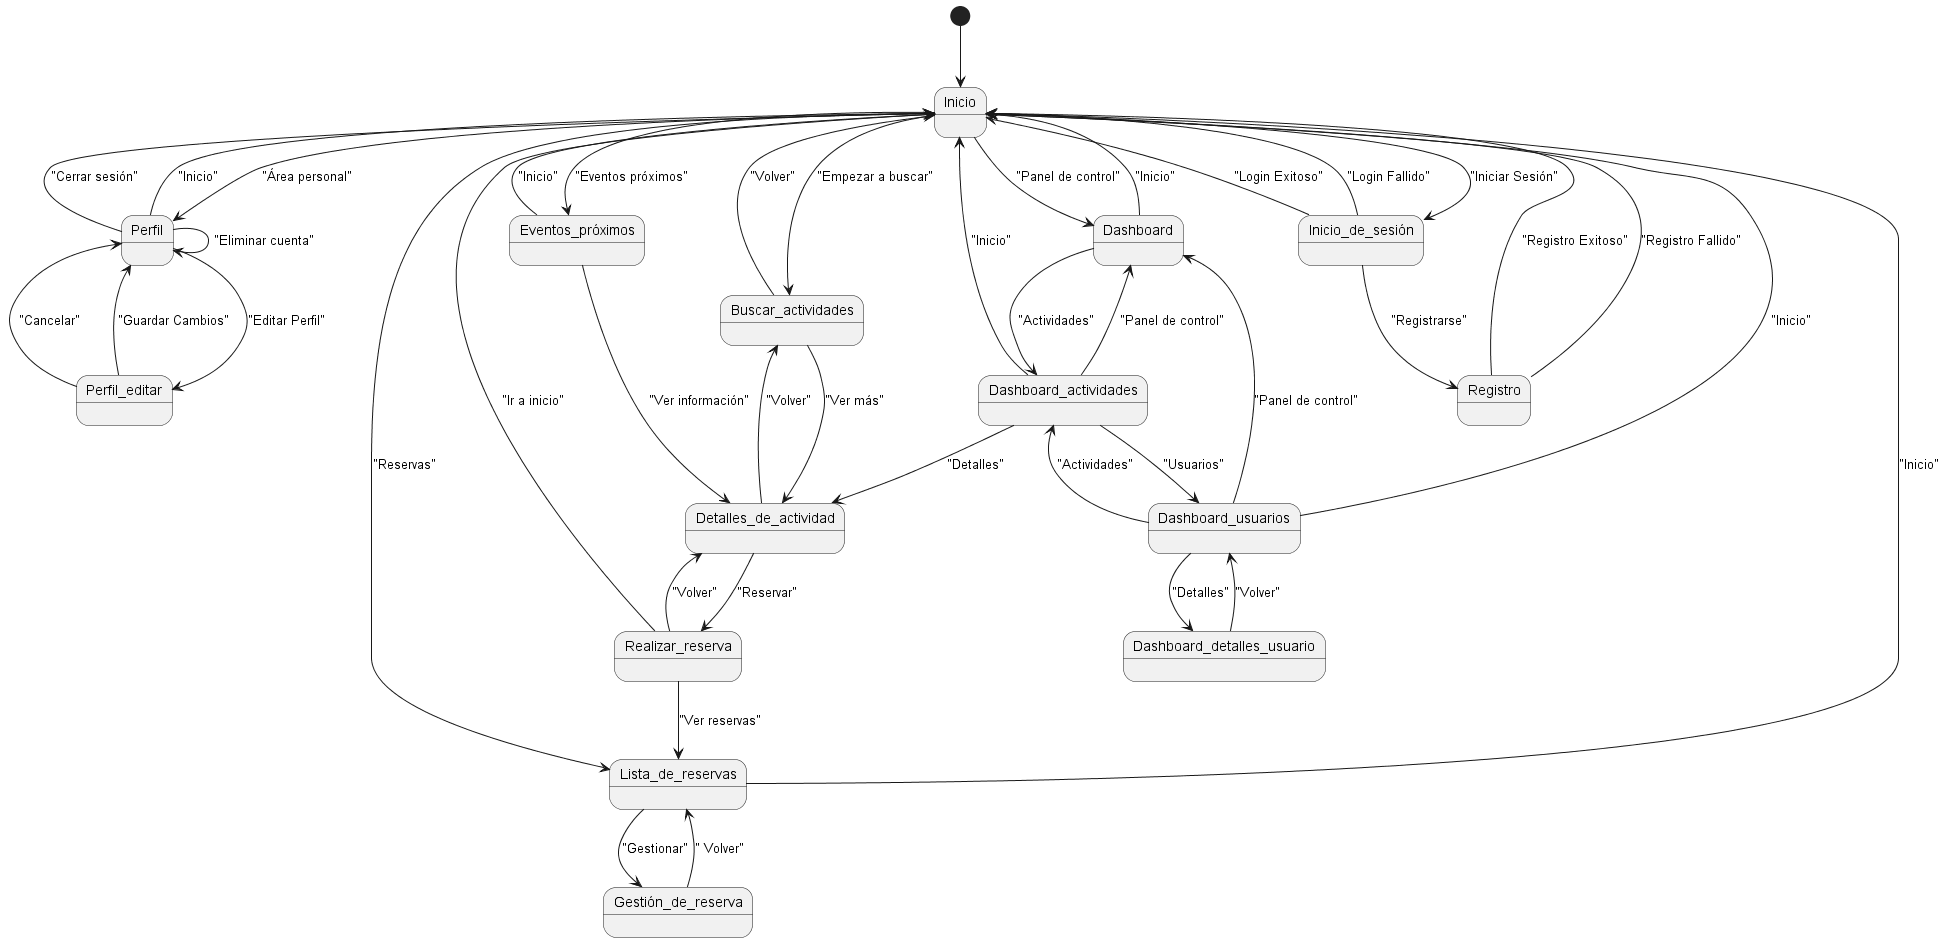
\includegraphics[width=1\linewidth]{5-AnalisisDelSistemaDeInformacion/Navegabilidad/diagrama.png}
	\caption{Diagrama de las relaciones entre los subsistemas}
	\label{fig:diagrama}
\end{figure}
\section{Especificación del plan de pruebas}
En esta sección se describe el plan de pruebas que se llevará a cabo para garantizar la calidad y funcionalidad del sistema. Se realizarán pruebas unitarias, pruebas de integración y pruebas de usabilidad.
\subsection{Pruebas unitarias}
Las pruebas unitarias se centran en validar el correcto funcionamiento de cada componente individual del sistema. Para ello:
\begin{itemize}
	\item Se definirán casos de prueba específicos para cada función o método.
	\item Cada caso de prueba verificará que los resultados obtenidos sean los esperados bajo diferentes condiciones.
	\item Se empleará el framework de pruebas unitarias Jest, conocido por su eficacia en la detección de errores en etapas tempranas del desarrollo.
	\item Estas pruebas se ejecutarán de manera automatizada para asegurar la repetibilidad y consistencia de los resultados.
\end{itemize}
\subsection{Pruebas de integración}
Para verificar la correcta integración entre los diferentes módulos de la funcionalidad de reservas de actividades, se realizarán pruebas de integración centradas en la creación de reservas, dado que es la funcionalidad principal y la que más relaciones entre módulos presenta.
Las pruebas se llevarán a cabo en un entorno de pruebas similar al de producción utilizando herramientas de automatización como Cypress.
Se comprobará la conexión entre el módulo de usuario y el módulo de reservas para asegurar que un usuario autenticado puede crear una reserva;
la conexión entre el módulo de actividades y el módulo de reservas para verificar que las actividades disponibles se cargan y pueden ser seleccionadas correctamente;
y la interacción entre el módulo de reservas y la base de datos para garantizar que la información de la reserva se almacena y recupera adecuadamente.

Además se realizarán pruebas manuales para comprobar la correcta visualización de la información de la reserva en la interfaz de usuario y la correcta actualización de la base de datos tras la realización de una reserva.
\subsection{Pruebas de usabilidad}
Las pruebas de usabilidad están diseñadas para evaluar la experiencia del usuario al interactuar con el sistema. Estas pruebas se centrarán en la facilidad de uso, la eficiencia y la satisfacción del usuario. El enfoque principal será la realización de un cuestionario estructurado después de que los participantes completen una serie de tareas específicas en la aplicación. A continuación se detalla el plan para estas pruebas:
\\[1ex]
\textbf{Selección de Participantes:}
\\[1ex]
Se seleccionarán de 3 a 5 personas que representen el público objetivo de la aplicación.
Los participantes deben tener diferentes niveles de experiencia con aplicaciones similares para obtener una variedad de perspectivas.
Tareas a Realizar:
\begin{enumerate}
	\item Registrarse en la aplicación
	\item Cerrar sesión
	\item Iniciar sesión
	\item Buscar actividades
	\item Filtrar actividades por texto
	\item Filtrar actividades por rango/precio/personas
	\item Borrar filtros de búsqueda
	\item Ver Detalles de una actividad
	\item Reservar una actividad
	\item Cancelar una reserva
	\item Añadir una valoración
	\item Editar una valoración
	\item Eliminar una valoración
	\item Ver datos personales
	\item Editar datos personales
	\item Cambiar la contraseña
	\item Cambiar el tema de la aplicación
	\item Cambiar el idioma de la aplicación
	\item Eliminar la cuenta
\end{enumerate}

Al ser una aplicación web y móvil, se realizarán pruebas en ambas plataformas para evaluar la consistencia y la usabilidad en diferentes dispositivos.
A su vez, también se evaluarán tareas de administración para los usuarios con rol de administrador y tareas de guía para los usuarios con rol de guía.

\textbf{Cuestionario de Usabilidad:}
\\[1ex]
Después de completar cada tarea, los participantes responderán a preguntas sobre la facilidad de realizar la tarea y cualquier problema que hayan encontrado.
Se recopilará feedback cualitativo y cuantitativo para evaluar la usabilidad general de la aplicación.